\documentclass[12pt]{article}
\usepackage{ctex}
\usepackage{graphicx}
\usepackage{subfigure}
\usepackage{caption}
\usepackage{float}
\usepackage{physics}
\usepackage{amsmath}
\usepackage{geometry}
\geometry{left=2.5cm,right=2.5cm,top=2.5cm,bottom=2.5cm}
\title{Quantum Many-particle Systems (Note)}

\graphicspath{{figures/}}

\begin{document}
\maketitle
\section{Second Quantization and Coherent States}

We define a state $\ket{\vec{r}\sigma\tau}$, which is a state of the particle 
localized at point $\vec{r}$, with a projection of the spin $\sigma$ 
and isospin $\tau$. These states span the Hilbert space of the particle:
\begin{equation*}
    \sum_{\sigma=\pm\frac{1}{2}}\sum_{\tau=\pm\frac{1}{2}}
    \int d^3r\ket{\vec{r}\sigma\tau}\bra{\vec{r}\sigma\tau}=1
\end{equation*} 
where we suppose the particle has only two eigenvalues of isospin $\tau$, 
like a proton or neutron.

Their overlap is given by:

\begin{equation*}
    \bra{\vec{r}\sigma\tau}\ket{\vec{r}'\sigma'\tau'}=\delta_{\sigma\sigma'}
    \delta_{\tau\tau'}\delta^3(\vec{r}-\vec{r}')
\end{equation*}
We order:
\begin{equation*}
    \ket{x}\equiv\ket{\vec{r}\sigma\tau}
\end{equation*}
and
\begin{equation*}
    \int dx=\sum_{\sigma=\pm\frac{1}{2}}\sum_{\tau=\pm\frac{1}{2}}\int d^3r;
\end{equation*}
\begin{equation*}
    \delta(x-x')=\delta_{\sigma\sigma'}\delta_{\tau\tau'}
    \delta^3(\vec{r}-\vec{r}')
\end{equation*}
Using this notation, we can write:
\begin{equation*}
    \int dx\ket{x}\bra{x}=1
\end{equation*}
and
\begin{equation*}
    \bra{x}\ket{x'}=\delta(x-x')
\end{equation*}
For desicribing a system with N particles, define Hilbert space $\mathcal{H}_N$:
\begin{equation*}
    \mathcal{H}_N=\mathcal{H}\otimes\mathcal{H}\otimes\dots\otimes\mathcal{H}
\end{equation*}
\begin{equation*}
    |\alpha_1\dots\alpha_N)=\ket{\alpha_1}\otimes\ket{\alpha_2}\otimes\dots
    \otimes\ket{\alpha_N}
\end{equation*}
To distinguish Bosons and Fermions, and for convenience, we shall adopt the following
unified notation:
\begin{equation*}
    \psi(\vec{r}_{P1},\vec{r}_{P2},\dots,\vec{r}_{PN})
    =\zeta^P\psi(\vec{r}_1,\vec{r}_2,\dots,\vec{r}_N)
\end{equation*}
A wave function belongs to the Hilbert space of N Bosons $\mathcal{B}_N$, or the 
Hilbert space of N Fermions $\mathcal{F}_N$, if $\zeta$ equals to $+1$ or $-1$.

The symmetrization operator $\mathcal{P}_B$ and the antisymmetrization operator 
$\mathcal{P}_F$:
\begin{equation*}
    \mathcal{P}_{\{\substack{\small B\\\small F}\}}\psi(\vec{r}_1,\vec{r}_2,\dots\vec{r}_N)
    =\frac{1}{N!}\sum_P\zeta^P\psi(\vec{r}_{P1},\vec{r}_{P2},\dots,\vec{r}_{PN})
\end{equation*}
For Bosons:
\begin{equation*}
    \mathcal{P}_B\psi(\vec{r}_1,\vec{r}_2)=\frac{1}{2}[\psi(\vec{r}_1,\vec{r}_2)
    +\psi(\vec{r}_2,\vec{r}_1)];
\end{equation*}
and for Fermions:
\begin{equation*}
    \mathcal{P}_F\psi(\vec{r}_1,\vec{r}_2)=\frac{1}{2}[\psi(\vec{r}_1,\vec{r}_2)
    -\psi(\vec{r}_2,\vec{r}_1)]
\end{equation*}
The operator $\mathcal{P}_{\{\substack{\small B\\\small F}\}}$ may be shown to be a 
projector as follows:
\begin{equation*}
    \begin{split}
        \mathcal{P}^2_{\{\substack{\small B\\\small F}\}}\psi(\vec{r}_1,\dots\vec{r}_N)
        &=\frac{1}{N!}\frac{1}{N!}\sum_{P}\sum_{P'}\zeta^P\zeta^{P'}
        \psi(\vec{r}_{P'P1},\vec{r}_{P'P2},\dots,\vec{r}_{P'PN})\\
        &=\frac{1}{N!}\sum_P\Big[\frac{1}{N!}\sum_Q\zeta^Q
        \psi(\vec{r}_{Q1},\vec{r}_{Q2},\dots,\vec{r}_{QN})\Big]\\
        &=\frac{1}{N!}\sum_P\mathcal{P}_{\{\substack{\small B\\\small F}\}}
        \psi(\vec{r}_1,\dots\vec{r}_N)\\
        &=\mathcal{P}_{\{\substack{\small B\\\small F}\}}\psi(\vec{r}_1,\dots\vec{r}_N)
    \end{split}
\end{equation*}
These operators project $\mathcal{H}_N$ onto the Hilbert space of Bosons $\mathcal{B}_N$ 
and the Hilbert space of Fermions $\mathcal{F}_N$:
\begin{equation*}
    \begin{split}
        &\mathcal{B}_N=\mathcal{P}_B\mathcal{H}_N\\
        &\mathcal{F}_N=\mathcal{P}_F\mathcal{H}_N
    \end{split}
\end{equation*}
Thus, a system of N Bosons or Fermions can be represented as follows:
\begin{equation*}
    \begin{split}
        |\alpha_1\dots\alpha_N\}&=\sqrt{N!}\mathcal{P}_{\{\substack{\small B\\\small F}\}}
        |\alpha_1\dots\alpha_N)\\
        &=\frac{1}{\sqrt{N!}}\sum_P\zeta^P\ket{\alpha_{P_1}}\otimes\dots\otimes
        \ket{\alpha_{PN}}
    \end{split}
\end{equation*}
It follows that if $|\alpha_1\dots\alpha_N)$ is a basis of $\mathcal{H}_N$, 
then $\mathcal{P}_{\{\substack{\small B\\\small F}\}}|\alpha_1\dots\alpha_N)$ is 
a basis of $\mathcal{B}_N$ or $\mathcal{F}_N$。
The normalized states is written as $\ket{\alpha_1\dots\alpha_N}$:
\begin{equation*}
    \ket{\alpha_1\dots\alpha_N}=\frac{1}{\sqrt{\prod_\alpha n_\alpha!}}
    |\alpha_1\dots\alpha_N\}
\end{equation*}
where $n_\alpha$ is the occupation number of each state.

Let $\mathcal{O}$ be an arbitrary operator in $\mathcal{B}_N$ or $\mathcal{F}_N$, 
For any states, and any permutation:
\begin{equation*}
    (\alpha_{P1}\dots\alpha_{PN}|\mathcal{O}|\alpha'_{P1}\dots\alpha'_{PN})
    =(\alpha_1\dots\alpha_N|\mathcal{O}|\alpha'_1\dots\alpha'_N)
\end{equation*}
An operator $\hat{U}$ is a one-body operator if:
\begin{equation*}
    \hat{U}|\alpha_1\dots\alpha_N)=\sum_{i=1}^{N}\hat{U}_i|\alpha_1\dots\alpha_N)
\end{equation*}
For example, the kinetic operator $\hat{T}$ in the $\{\vec{p}\}$ basis acts as:
\begin{equation*}
    \hat{T}|\vec{p}_1\dots\vec{p}_N)=\sum_{i=1}^{N}\frac{\hat{\vec{p}}^2_i}{2m}
    |\vec{p}_1\dots\vec{p}_N)
\end{equation*}
and a local potential operator $\hat{W}$ in $\{x\}$ basis acts as:
\begin{equation*}
    \hat{W}|x_1\dots x_N)=\sum_{i=1}^NW(x_i)|x_1\dots x_N)
\end{equation*}
Similarly, an operator $\hat{V}$ is a two-body operator if:
\begin{equation*}
    \hat{V}|\alpha_1\dots \alpha_N)=\sum_{1\leq i<j\leq N}\hat{V}_{ij}
    |\alpha_1\dots \alpha_N)
\end{equation*}
A two-body interaction $\hat{V}$ is said to be local, or to be velocity independent, 
when it is diagonal in configuration space(and spin and isospin, if appropriate).
\begin{equation*}
    (\vec{r}_1\vec{r}_2|\hat{V}|\vec{r}_3\vec{r}_4)=\delta(\vec{r}_1-\vec{r}_3)
    \delta(\vec{r}_2-\vec{r}_4)v(\vec{r}_1-\vec{r}_2)
\end{equation*}
Notice that $\hat{V}_{ij}=\hat{V}_{ji}$. In this case, we have
\begin{equation*}
    \hat{V}|\alpha_1\dots \alpha_N)=\frac{1}{2}\sum_{1\le i\neq j\le N}
    v(\vec{r}_1-\vec{r}_2)|\alpha_1\dots \alpha_N)
\end{equation*}
In general, we define an n-body operator $\hat{R}$ which acts on 
$\ket{\alpha_1\dots\alpha_N}$ as:
\begin{equation*}
    \hat{R}|\alpha_1\dots\alpha_N)=\frac{1}{n!}\sum_{1\leq i_1\neq i_2\neq\dots
    \neq i_n\leq N}\hat{R}_{i_1i_2... i_n}|\alpha_1\dots\alpha_N).
\end{equation*} 
The creation operator: $a^\dagger_\lambda$
\begin{equation*}
    a^\dagger_\lambda|\lambda_1\dots\lambda_N\}\equiv|\lambda\lambda_1\dots\lambda_N\}
\end{equation*}
In order to allow the creation operator $a^\dagger_\lambda$ and annihilation operator 
$a_\lambda$ to operate within one space, we define the Fock space 
$\mathcal{B}$ and $\mathcal{F}$ as direct sum of Boson or Fermion spaces:
\begin{equation*}
    \mathcal{B}=\mathcal{B}_0\oplus\mathcal{B}_1\oplus\mathcal{B}_2\oplus\dots
    =\oplus_{n=0}^{\infty}\mathcal{B}_n
\end{equation*}
\begin{equation*}
    \mathcal{F}=\mathcal{F}_0\oplus\mathcal{F}_1\oplus\mathcal{F}_2\oplus\dots
    =\oplus_{n=0}^{\infty}\mathcal{F}_n
\end{equation*}
Where by defination:
\begin{equation*}
    \begin{split}
        &\mathcal{B}_0=\mathcal{F}_0=\ket{0}\\
        &\mathcal{B}_1=\mathcal{F}_1=\mathcal{H}
    \end{split}
\end{equation*} 
The closure relation in the Fock space may be written:
\begin{equation*}
    1=\ket{0}\bra{0}+\sum_{N=1}^\infty\frac{1}{N!}\sum_{\lambda_1\dots\lambda_N}
    |\lambda_1\dots\lambda_N\}\{\lambda_1\dots\lambda_N|
\end{equation*}
The annihilation operator $a_\lambda$. For Bosons:
\begin{equation*}
    a_\lambda\ket{n_{\beta_1}n_{\beta_2}\dots n_{\lambda}\dots}
    =\sqrt{n_\lambda}\ket{n_{\beta_1}n_{\beta_2}\dots (n_{\lambda}-1)\dots},
\end{equation*}
which is expressed in occupation number representation.
For Fermions:
\begin{equation*}
    a_\lambda\ket{\beta_1\dots\beta_n}=\left\{
        \begin{split}
            &(-1)^{i-1}\ket{\beta_1\dots\hat{\beta}_i\dots\beta_n},\ 
            if\ \ket{\lambda}\ is\ occupied\\
            &0,\qquad\qquad\qquad\qquad\qquad\quad if\ \ket{\lambda}\ is\ unoccupied.
        \end{split}   
    \right.
\end{equation*}
\begin{equation*}
    \begin{split}
        a^{\dagger}_{\tilde{\alpha}}|\alpha_1\cdots\alpha_n\}&=\sum_{\alpha}
        \langle\alpha|\tilde{\alpha}\rangle|\alpha\alpha_1\dots\alpha_n\}\\
        &=\sum_\alpha\langle\alpha|\tilde{\alpha}\rangle a_\alpha^\dagger
        |\alpha_1\dots\alpha_n\}
    \end{split}
\end{equation*}
The creation operators satisfy the operator equation:
\begin{equation*}
    a^\dagger_{\tilde{\alpha}}=\sum_\alpha\langle\alpha|\tilde{\alpha}\rangle a_\alpha^\dagger
\end{equation*}
and the annihilation operators satisfy the adjoint equation:
\begin{equation*}
    a_{\tilde{\alpha}}=\sum_\alpha\langle\alpha|\tilde{\alpha}\rangle a_\alpha
\end{equation*}
To represent the operator in the diagonal basis, we define the numnber operator 
$\hat{n}_\alpha$:
\begin{equation*}
    \hat{n}_\alpha=a^\dagger_\alpha a_\alpha
\end{equation*}
The operator $\hat{N}$ counts the total number of particles in a state:
\begin{equation*}
    \hat{N}=\sum_\alpha\hat{n}_\alpha=\sum_\alpha a^\dagger_\alpha a_\alpha
\end{equation*}
$\hat{U}$ is a one-body operator, and is diagonal in the orthonormal basis 
$\ket{\alpha}$.
\begin{equation*}
    U_\alpha=\bra{\alpha}U\ket{\alpha}
\end{equation*}
We can write:
\begin{equation*}
    \begin{split}
        \{\alpha'_1\dots\alpha'_N|U|\alpha_1\dots\alpha_N\}&=
        \sum_P\zeta^P\sum_{i=1}^N\prod_{k\neq1}\langle\alpha'_{Pk}|\alpha_k\rangle
        \bra{\alpha'_{Pi}}U\ket{\alpha_i}\\
        &=\left(\sum_{i=1}^NU_{\alpha_i}\right)
        \{\alpha'_1\dots\alpha'_N|\alpha_1\dots\alpha_N\}\\
        &=\{\alpha'_1\dots\alpha'_N|\sum_\alpha U_\alpha \hat{n}_\alpha|
        \alpha_1\dots\alpha_N\}
    \end{split}
\end{equation*}
Since the equality holds for any states, we obtain the operator equation:
\begin{equation*}
    \hat{U}=\sum_\alpha U_\alpha\hat{n}_\alpha
    =\sum_\alpha \bra{\alpha}U\ket{\alpha}a^\dagger_\alpha a_\alpha
\end{equation*}
$\hat{V}$ is a diagonal two-body operator
\begin{equation*}
    V_{\alpha\beta}=(\alpha\beta|V|\alpha\beta)
\end{equation*}
$\hat{P}_{\alpha\beta}$ is an operator which counts the number of pairs of particles 
in the states $\ket{\alpha}$ and $\ket{\beta}$. If $\ket{\alpha}$ and $\ket{\beta}$ 
are different, the number of pairs is $n_\alpha n_\beta$ whereas 
if $\ket{\alpha}=\ket{\beta}$, the number of pairs is $n_\alpha (n_\beta-1)$. 
Hence, the operator which counts pairs may be written
\begin{equation*}
    \hat{P}_{\alpha\beta}=\hat{n}_\alpha\hat{n}_\beta-\delta_{\alpha\beta}\hat{n}_\alpha
\end{equation*}
Notice that
\begin{equation*}
    a_\alpha a^\dagger_\beta-\zeta a^\dagger_\beta a_\alpha=\delta_{\alpha\beta}
\end{equation*}
Thus $\hat{P}_{\alpha\beta}$ can be written in terms of creation and annihilation 
operators
\begin{equation*}
    \begin{split}
        \hat{P}_{\alpha\beta}&=a^\dagger_\alpha a_\alpha a^\dagger_\beta a_\beta-
        \delta_{\alpha\beta}a^\dagger_\alpha a_\alpha\\
        &=a^\dagger_\alpha\zeta a^\dagger_\beta a_\alpha a_\beta
        +\delta_{\alpha\beta}a^\dagger_\alpha a_\beta
        -\delta_{\alpha\beta}a^\dagger_\alpha a_\alpha\\
        &=a^\dagger_\alpha a^\dagger_\beta a_\beta a_\alpha
    \end{split}
\end{equation*}
Using this operator, the action of two-body operator $\hat{V}$ can be written as:
\begin{equation*}
    \{\alpha'_1\dots\alpha'_n|\hat{V}|\alpha_1\dots\alpha_n\}=\{\alpha'_1\dots\alpha'_n|
    \frac{1}{2}\sum_{\alpha\beta}V_{\alpha\beta}\hat{P}_{\alpha\beta}|\alpha_1\dots\alpha_n\}
\end{equation*}
Hence we obtain the operator equation:
\begin{equation*}
    \hat{V}=\frac{1}{2}\sum_{\alpha\beta}V_{\alpha\beta}\hat{P}_{\alpha\beta}
    =\frac{1}{2}\sum_{\alpha\beta}(\alpha\beta|V|\alpha\beta)
    a^\dagger_\alpha a^\dagger_\beta a_\beta a_\alpha
\end{equation*}
The general expression for a two-body potential is
\begin{equation*}
    \hat{V}=\frac{1}{2}\sum_{\lambda\mu\nu\rho}(\lambda\mu|V|\nu\rho)
    a^\dagger_\lambda a^\dagger_\mu a_\nu a_\rho
\end{equation*}
The preceding derivations for one and two-body operators may be straightforwardly 
generalized to n-body operators, with the result:
\begin{equation*}
    \hat{R}=\frac{1}{n!}\sum_{\lambda_1\dots\lambda_n}\sum_{\mu_1\dots\mu_n}
    (\lambda_1\dots\lambda_n|\hat{R}|\mu_1\dots\mu_n)a^\dagger_{\lambda_1}
    \dots a^\dagger_{\lambda_n}a_{\mu_1}\dots a_{\mu_n}
\end{equation*}
\subsection*{Coherent States}
Coherent states are defined as eigenstates of annihilation operators. For an arbitrary 
state $\ket{\phi}$ in Fock space, we can expand it as:
\begin{equation*}
    \ket{\phi}=\sum_{n=0}^{\infty}\sum_{\alpha_1\dots\alpha_n}
    \phi_{\alpha_1\dots\alpha_n}\ket{\alpha_1\dots\alpha_n}
\end{equation*}
Assuming $\ket{\phi}$ is a eigenstate of the annihilation operators, then
\begin{equation*}
    a_\alpha\ket{\phi}=\phi_\alpha\ket{\phi}
\end{equation*}
The commutation and anticommutation relations of Bosons and Fermions imply the 
corresponding relations for the eigenvalues:
\begin{equation*}
    \left[\phi_\alpha,\phi_\beta\right]_{-\zeta}=0
\end{equation*}
For Fermions, the eigenvalues anticommute, we will need to define anticommute 
variables called Grassmann numbers. However, for Bosons, the eigenvalues commute
and we can just proceed straightforwardly using ordinary numbers.

We shall start with Bosons coherent states. A Boson coherent state can be expanded 
in occupation number representation as
\begin{equation*}
    \ket{\phi}=\sum_{n_{\alpha_1}\dots n_{\alpha_p}}
    \phi_{n_{\alpha_1}\dots n_{\alpha_p}}\ket{n_{\alpha_1}\dots n_{\alpha_p}}
\end{equation*}
According to the eigenequation, the relations on coefficients for all $\{n_\alpha\}$ 
is
\begin{equation*}
    \sqrt{n_{\alpha_i}}\phi_{n_{\alpha_1}\dots n_{\alpha_i}\dots}
    =\phi_{\alpha_i}\phi_{n_{\alpha_1}\dots (n_{\alpha_i}-1)\dots}
\end{equation*}
By recursion, we obtain
\begin{equation*}
    \phi_{n_{\alpha_1}n_{\alpha_2}\dots n_{\alpha_i}}=
    \frac{\phi^{n_{\alpha_1}}_{\alpha_1}\phi^{n_{\alpha_2}}_{\alpha_2}\dots
    \phi^{n_{\alpha_i}}_{\alpha_i}\dots}{\sqrt{n_{\alpha_1}!}\sqrt{n_{\alpha_2}!}
    \dots\sqrt{n_{\alpha_i}!}\dots}
\end{equation*}
\begin{equation*}
    \ket{n_{\alpha_1}n_{\alpha_2}\dots n_{\alpha_p}\dots}=
    \frac{(a^\dagger_{\alpha_1})^{n_{\alpha_1}}}{\sqrt{n_{\alpha_1}!}}
    \frac{(a^\dagger_{\alpha_2})^{n_{\alpha_2}}}{\sqrt{n_{\alpha_2}!}}\dots
    \frac{(a^\dagger_{\alpha_p})^{n_{\alpha_p}}}{\sqrt{n_{\alpha_p}!}}\dots\ket{0}
\end{equation*}
Hence we finally obtain:
\begin{equation*}
    \begin{split}
        \ket{\phi}&=\sum_{n_{\alpha_1},n_{\alpha_2}\dots n_{\alpha_p}}
        \frac{(\phi_{\alpha_1}a^\dagger_{\alpha_1})^{n_{\alpha_1}}}{n_{\alpha_1}!}
        \frac{(\phi_{\alpha_2}a^\dagger_{\alpha_2})^{n_{\alpha_2}}}{n_{\alpha_2}!}
        \dots\frac{(\phi_{\alpha_p}a^\dagger_{\alpha_p})^{n_{\alpha_p}}}
        {n_{\alpha_p}!}\ket{0}\\
        &=\exp\Big[\sum_\alpha\phi_\alpha a^\dagger_\alpha\Big]\ket{0}\\
        \bra{\phi}&=\bra{0}\exp\Big[\sum_\alpha\phi^*_\alpha a_\alpha\Big]
    \end{split}
\end{equation*}
The action of a creation operator on a coherent state is given by
\begin{equation*}
    a^\dagger_\alpha\ket{\phi}=a^\dagger_\alpha
    \exp\Big[\sum_\alpha\phi_\alpha a^\dagger_\alpha\Big]\ket{0}
    =\frac{\partial}{\partial\phi_\alpha}\ket{\phi}
\end{equation*}
with the adjoint relation:
\begin{equation*}
    \bra{\phi}a_\alpha=\frac{\partial}{\partial\phi^*}\bra{\phi}
\end{equation*}
The overlap of two coherents is given by 
\begin{equation*}
    \braket*{\phi}{\phi'}=\exp\Big[\sum_\alpha\phi_\alpha^*\phi'_\alpha\Big]
\end{equation*}
Coherent states are overcomplete in Fock space. Any state $\ket{\psi}$ can be 
represented as:
\begin{equation*}
    \ket{\psi}=\int \prod_\alpha\frac{d\phi^*_\alpha d\phi_\alpha}{2\pi i}
    e^{-\sum_\alpha \phi_\alpha^*\phi_\alpha}\psi(\phi^*)\cdot\ket{\phi}
\end{equation*}
where 
\begin{equation*}
    \frac{d\phi^*_\alpha d\phi_\alpha}{2\pi i}=
    \frac{d({\rm Re}\phi_\alpha)d({\rm Im}\phi_\alpha)}{\pi}
\end{equation*}
and
\begin{equation*}
    \psi(\phi^*)=\braket*{\phi}{\psi}
\end{equation*}
is the coherent state representation of the state $\ket{\psi}$.
According to equations above, we find:
\begin{equation*}
    \bra{\phi}a_\alpha\ket{f}=\frac{\partial}{\partial\phi_\alpha^*}f(\phi^*)
\end{equation*}
\begin{equation*}
    \bra{\phi}a^\dagger_\alpha\ket{f}=\phi_\alpha^* f(\phi^*)
\end{equation*}
Hence we can write the annihilation and creation operator in coherent state 
representation:
\begin{equation*}
    a_\alpha=\frac{\partial}{\partial\phi_\alpha^*}
\end{equation*}
\begin{equation*}
    a^\dagger_\alpha=\phi^*_\alpha
\end{equation*}
which is consistent with the Boson commutation rules:
\begin{equation*}
    [\phi^*_\alpha,\phi^*_\beta]=\bigg[\frac{\partial}{\partial\phi^*_\alpha},
    \frac{\partial}{\partial\phi^*_\beta}\bigg]=0
\end{equation*}
\begin{equation*}
    \bigg[\frac{\partial}{\partial\phi^*_\alpha},\phi^*_\beta\bigg]
    =\delta_{\alpha\beta}
\end{equation*}
The projection of the schrodinger equation:
\begin{equation*}
    H(\phi^*_\alpha,\frac{\partial}{\partial\phi^*_\alpha})\psi(\phi^*)
    =E\psi(\phi^*)
\end{equation*}
For a stantard Hamiltonian eith one and two-body operators, it reads:
\begin{equation*}
    \left(\sum_{\alpha,\beta}T_{\alpha\beta}\phi^*_\alpha
    \frac{\partial}{\partial\phi^*_\beta}+\frac{1}{2}
    \sum_{\alpha\beta\gamma\delta}(\alpha\beta|v|\gamma\delta)
    \phi^*_\alpha\phi^*_\beta\frac{\partial}{\partial\phi^*_\gamma}
    \frac{\partial}{\partial\phi^*_\delta}\right)\psi(\phi^*)=E\psi(\phi^*)
\end{equation*}
\subsection*{Grassmann Algebra}
Algebras of anticommuting numbers are called Grassmann algebras. A Grassmann 
algebra is defined by a set of generators $\{\xi_\alpha\}$, $\alpha=1,\dots,n$. 
These generators anticommute:
\begin{equation*}
    \xi_\alpha\xi_\beta+\xi_\beta\xi_\alpha=0
\end{equation*}
Thus $\xi_\alpha^2=0$. 
The basis of the Grassmann algebra is made of all distinct products of the 
generators. Thus, a number in Grassmann algebra is a linear combination with 
complex coefficients of the numbers $\{1,\xi_{\alpha_1},\xi_{\alpha_1}
\xi_{\alpha_2},\dots,\xi_{\alpha_1}\xi_{\alpha_2}\dots\xi_{\alpha_n}\}$. The 
dimension of a Grassmann algebra with $n$ generators is $2^n$.

Conjugation in a Grassmann algebra:
\begin{equation*}
    (\xi_\alpha)^*=\xi_\alpha^*
\end{equation*}
\begin{equation*}
    (\xi_\alpha^*)^*=\xi_\alpha
\end{equation*}
If $\lambda$ is a complex number,
\begin{equation*}
    (\lambda\xi_\alpha)^*=\lambda^*\xi_\alpha^*
\end{equation*}
and for any product of generators,
\begin{equation}
    (\xi_{\alpha_1}\xi_{\alpha_2}\dots\xi_{\alpha_n})^*=
    \xi_{\alpha_n}^*\xi_{\alpha_{n-1}}^*\dots\xi_{\alpha_1}^*
\end{equation}
Consider a Grassmann algebra with two generators $\xi$ and $\xi^*$, and is 
generated by the four numbers: $\{1,\xi,\xi^*,\xi^*\xi\}$. Because of it's 
property, any function $f$ defined on this algebra is a linear function.
\begin{equation*}
    f(\xi)=f_0+f_1\xi
\end{equation*}
The coherent state representation of an operator in the Grassmann algebra will 
be a function and must have the form:
\begin{equation*}
    A(\xi^*,\xi)=a_0+a_1\xi+\bar{a_1}\xi^*+a_{12}\xi^*\xi
\end{equation*}
As for ordinary complex functions, a derivative operator can be defined for 
Grassmann variable functions.
\begin{equation*}
    \frac{\partial}{\partial\xi}(\xi^*\xi)=
    \frac{\partial}{\partial\xi}(-\xi\xi^*)=-\xi^*
\end{equation*}
Notice that
\begin{equation*}
    \frac{\partial}{\partial\xi}\frac{\partial}{\partial\xi^*}A(\xi^*,\xi)=
    -\frac{\partial}{\partial\xi^*}\frac{\partial}{\partial\xi}A(\xi^*,\xi)
\end{equation*}
Thus the operators $\frac{\partial}{\partial\xi}$ and 
$\frac{\partial}{\partial\xi}$ anticommute.

We define integration over Grassmann variables as a linear mapping which has 
fundamental property of ordinary integrals over functions vanishing at infinity 
that the integral of an exact differential form is zero.
\begin{equation*}
    \begin{split}
        \int d\xi1=0\\
        \int d\xi\xi=1
    \end{split}
\end{equation*}
We can then define delta function in Grassmann algebra:
\begin{equation*}
    \begin{split}
        \delta(\xi,\xi')&=\int d\eta e^{-\eta(\xi-\xi')}\\
        &=\int d\eta[1-\eta(\xi-\xi')]\\
        &=-(\xi-\xi')
    \end{split}
\end{equation*}  
\begin{equation*}
    \begin{split}
        \int d\xi'\delta(\xi,\xi')f(\xi')&=-\int d\xi'(\xi-\xi')(f_0+f_1\xi')\\
        &=\int d\xi'(-f_0\xi+f_1\xi'\xi+f_0\xi')\\
        &=f_0+f_1\xi=f(\xi)
    \end{split}
\end{equation*}
We then define a scalar product of Grassmann functions by:
\begin{equation*}
    \braket*{f}{g}=\int d\xi^*d\xi e^{-\xi^*\xi}f^*(\xi)g(\xi^*)
\end{equation*}
With this defination, we see that:
\begin{equation*}
    \begin{split}
        \braket*{f}{g}&=\int d\xi^*d\xi(1-\xi^*\xi)(f_0^*+f_1^*\xi)(g_0+g_1\xi^*)\\
        &=f_0^*g_0+f_1^*g_1
    \end{split}
\end{equation*}
Grassmann functions have the structure of a Hilbert space.
The coefficients of a Fermion coherent state must be Grassmann numbers. In order 
to construct Fermion coherent states, we need enlarge the Fermion Fock space.

$\mathcal{G}$ is a Grassmann algebra with generators $\xi_\alpha$ for each 
annihilation operators $a_\alpha$ and $\xi^*_\alpha$ for each creation operators 
$a_\alpha^\dagger$. We then construct the generalized Fock space as the set of 
linear combinations of states in Fock space $\mathcal{F}$ with the coefficients 
in the Grassmann algebra  $\mathcal{G}$. Any vector $\ket{\psi}$ in the generalized 
Fock space can be expanded as:
\begin{equation*}
    \ket{\psi}=\sum_\alpha\chi_\alpha\ket{\phi_\alpha}
\end{equation*} 
where $\chi_\alpha$ are Grassmann numbers and $\ket{\phi_\alpha}$ are vectors 
in Fock space $\mathcal{F}$. We require that:
\begin{equation*}
    \{\tilde{\xi},\tilde{a}\}=0
\end{equation*}
and
\begin{equation*}
    (\tilde{\xi}\tilde{a})^\dagger=\tilde{a}^\dagger\tilde{\xi}^*
\end{equation*}
We now define a Fermion coherent state $\ket{\xi}$ analogous to Boson coherent 
state:
\begin{equation*}
    \begin{split}
        \ket{\xi}&=\exp\Big[-\sum_\alpha\xi_\alpha a^\dagger_\alpha\Big]\ket{0}\\
        &=\prod_\alpha(1-\xi_\alpha a^\dagger_\alpha)\ket{0}
    \end{split}
\end{equation*}
\begin{equation*}
    \begin{split}
        a_\alpha(1-\xi_\alpha a^\dagger_\alpha)\ket{0}&=\xi_\alpha\ket{0}\\
        &=\xi_\alpha(1-\xi_\alpha a^\dagger_\alpha)\ket{0}
    \end{split}
\end{equation*}
Thus
\begin{equation*}
    \begin{split}
        a_\alpha\ket{\xi}&=a_\alpha\prod_\alpha(1-\xi_\alpha a^\dagger_\alpha)\ket{0}\\
        &=\xi_\alpha\ket{\xi}
    \end{split}
\end{equation*}
Similarly, the adjoint of the coherent state is 
\begin{equation*}
    \bra{\xi}=\bra{0}\exp\Big[-\sum_\alpha a_\alpha\xi_\alpha^*\Big]
    =\bra{0}\exp\Big[\sum_\alpha\xi_\alpha^*a_\alpha\Big]
\end{equation*}
and
\begin{equation*}
    \bra{\xi}a^\dagger_\alpha=\bra{\xi}\xi^*_\alpha
\end{equation*}
\begin{equation*}
    a^\dagger_\alpha\ket{\xi}=-\frac{\partial}{\partial\xi_\alpha}\ket{\xi}
\end{equation*}
\begin{equation*}
    \bra{\xi}a_\alpha=\frac{\partial}{\partial\xi^*_\alpha}\bra{\xi}
\end{equation*}
The overlap of two coherent states is calculated as:
\begin{equation*}
    \begin{split}
        \braket*{\xi}{\xi'}&=\bra{0}\prod_\alpha(1+\xi^*_\alpha a_\alpha)
        (1-\xi_\alpha a_\alpha^\dagger)\ket{0}\\
        &=\prod_\alpha(1+\xi_\alpha^*\xi_\alpha)\\
        &=\exp\Big[\sum_\alpha\xi^*_\alpha\xi_\alpha\Big]
    \end{split}
\end{equation*}
The closure relation can be written:
\begin{equation*}
    \int\prod_\alpha d\xi^*_\alpha d\xi_\alpha e^{-\sum_\alpha\xi^*_\alpha\xi_\alpha}
    \ketbra*{\xi}{\xi}=1
\end{equation*}
$\{\ket{n}\}$ is a complete set of states in Fock space. The trace of operator $A$ can 
be written:
\begin{equation*}
    \begin{split}
        \Tr A&=\sum_n\bra{n}A\ket{n}\\
        &=\int\prod_\alpha d\xi^*_\alpha d\xi_\alpha 
        e^{-\sum_\alpha\xi^*_\alpha\xi_\alpha}\sum_n\braket*{n}{\xi}\bra{\xi}A\ket{n}\\
        &=\int\prod_\alpha d\xi^*_\alpha d\xi_\alpha
        e^{-\sum_\alpha\xi^*_\alpha\xi_\alpha}\bra{-\xi}A\sum_n\ket{n}\braket*{n}{\xi}\\
        &=\int\prod_\alpha d\xi^*_\alpha d\xi_\alpha 
        e^{-\sum_\alpha\xi^*_\alpha\xi_\alpha}\bra{-\xi}A\ket{\xi}
    \end{split}
\end{equation*}
We can define a Grassmann coherent state representation analogous to the coherent state 
representation for Bosons.
\begin{equation*}
    \ket{\psi}=\int\prod_\alpha d\xi^*_\alpha d\xi_\alpha 
    e^{-\sum_\alpha\xi^*_\alpha\xi_\alpha}\psi(\xi^*)\ket{\xi}
\end{equation*} 
Where
\begin{equation*}
    \psi(\xi^*)=\braket*{\xi}{\psi}
\end{equation*}
analogous to Boson case:
\begin{equation*}
    \bra{\xi}a_\alpha\ket{\psi}=\frac{\partial}{\partial\xi^*_\alpha}\psi(\xi^*)
\end{equation*}
\begin{equation*}
    \bra{\xi}a^\dagger_\alpha\ket{\psi}=\xi^*_\alpha\psi(\xi^*)
\end{equation*}
The operators $a_\alpha$ and $a_\alpha^\dagger$ are represented as 
$\frac{\partial}{\partial\xi^*_\alpha}$ and $\xi^*_\alpha$ in the coherent states 
representation. The anticommutation relation is written:
\begin{equation*}
    \Big\{\frac{\partial}{\partial\xi^*_\alpha},\xi^*_\beta\Big\}=\delta_{\alpha\beta}
\end{equation*}
However, different from Boson, the expectation value of the number operator is not a 
real number. And it is meaningless to talk about the average number of particlas in a 
Fermion coherent state.
\begin{equation*}
    \frac{\bra{\xi}N\ket{\xi}}{\braket*{\xi}{\xi}}=\sum_\alpha\xi^*\xi
\end{equation*}
\subsection*{Guassian Integrals}
\begin{equation*}
    \int \frac{dx_1\dots dx_n}{(2\pi)^{\frac{n}{2}}}e^{-\frac{1}{2}x_iA_{ij}x_j+x_iJ_i}
    =[\det A]^{-\frac{1}{2}}e^{\frac{1}{2}J_iA^{-1}_{ij}J_j}
\end{equation*}
\begin{equation*}
    \int \prod_{i=1}^n\frac{dx_i^*dx_i}{2\pi i}e^{-x_i^*H_{ij}x_j+J_i^*x_i+J_ix_i^*}
    =[\det A]^{-1}e^{J_i^*H^{-1}_{ij}J_j}
\end{equation*}
\begin{equation*}
    \int d\xi^*d\xi e^{-\xi^*a\xi}=\int d\xi^*d\xi(1-\xi^*a\xi)=a
\end{equation*}
\section{General Formalism at Finite Temperature}
\subsection*{Functional Integral Formulation}
Consider a Matrix element of the evolution operator for a partical governed by 
Hamiltonian $\hat{H}(\hat{p},\hat{x})$
\begin{equation*}
    \mathcal{U}(x_ft_f,x_it_i)=\bra{x_f}e^{-\frac{i}{h}\hat{H}(t_f-t_i)}\ket{x_i}
\end{equation*}
Let the time interval $t_f-t_i$ be divided into M equal steps of size $\epsilon$:
\begin{equation*}
    \epsilon=\frac{t_f-t_i}{M}
\end{equation*}
with intermediate times denoted:
\begin{equation*}
    t_n=t_i+n\epsilon
\end{equation*}
with this notation:
\begin{center}
    $t_0\equiv t_i$ \ \ and \ \ $t_M\equiv t_f$
\end{center}
Use the same convention for coordinates:
\begin{center}
    $x_0\equiv x_i$ \ \ and \ \ $x_M\equiv x_f$
\end{center}
\begin{equation*}
    \begin{split}
        \mathcal{U}&=\bra{x_f}e^{-\frac{i}{h}\hat{H}(t_f-t_i)}\ket{x_i}\\
        &=\int\prod_{k=1}^{M-1}dx_k\bra{x_f}e^{-i\frac{\epsilon}{\hbar}\hat{H}}
        \ket{x_{M-1}}\bra{x_{M-1}}e^{-i\frac{\epsilon}{\hbar}\hat{H}}\ket{x_{M-2}}\\
        &\bra{{x_{M-2}}}\dots e^{-i\frac{\epsilon}{\hbar}\hat{H}}\ketbra*{x_1}{x_1}
        e^{-i\frac{\epsilon}{\hbar}\hat{H}}\ket{x_i}
    \end{split}
\end{equation*}
The infinitesimal evolution operator is written:
\begin{equation*}
    \bra{x_n}e^{-i\frac{\epsilon}{\hbar}\hat{H}(\hat{p},\hat{x})}\ket{x_{n-1}}
    =\int d^3p_n\braket*{x_n}{p_n}\bra{p_n}e^{-i\frac{\epsilon}{\hbar}
    \hat{H}(\hat{p},\hat{x})}\ket{x_{n-1}}
\end{equation*}
The Hamiltonian for a single particle in a potential:
\begin{equation*}
    H_v(\hat{p},\hat{x})=\frac{\hat{p}^2}{2m}+V(\hat{x})
\end{equation*}
We define an operator to be in normal form if all the $\hat{p}'$s appear to the left 
of all the $\hat{x}'$s. The result of reordering an operator 
$\mathcal{O}(\hat{p},\hat{x})$ into normal form is denoted as 
$:\mathcal{O}(\hat{p},\hat{x}):$.
\begin{equation*}
    :e^{-i\frac{\epsilon}{\hbar}H_v(\hat{p},\hat{x})}:
    =\sum_{n=0}(-i\frac{\epsilon}{\hbar})^n\sum_{k=0}^n\frac{1}{k!(n-k)!}
    (\frac{\hat{p}^2}{2m})^k(V(\hat{x}))^{n-k}
\end{equation*}
For any $\hat{H}(\hat{p},\hat{x})$ in normal form,
\begin{equation*}
    e^{-i\frac{\epsilon}{\hbar}H_v(\hat{p},\hat{x})}=
    :e^{-i\frac{\epsilon}{\hbar}H_v(\hat{p},\hat{x})}:+(-i\frac{\epsilon}{\hbar})^2
    \sum_{n=0}^\infty\frac{(-i\frac{\epsilon}{\hbar})^n}{(n+2)!}
    \left([H(\hat{p},\hat{x})]^{n+2}-:[H(\hat{p},\hat{x})]^{n+2}:\right)
\end{equation*}
For the special case: $H_v(\hat{p},\hat{x})=\frac{\hat{p}^2}{2m}+V(\hat{x})$, the 
leading correction is 
\begin{equation*}
    -\frac{\epsilon^2}{2\hbar^2}\Big[V,\frac{\hat{p}^2}{2m}\Big]
    =-\frac{\epsilon^2}{4m\hbar^2}(V''+2iV'\hat{p})
\end{equation*}
If the infinitesimal evolution operator is approximated by the normal-ordered 
evolution operator, the error is $\epsilon^2$ times an operator which may be 
expressed in terms of multiple commutators of the operators comprising the 
Hamiltonian. So that in limit $\epsilon\rightarrow0$, we are assured that 
$:e^{-i\frac{\epsilon}{\hbar}H(\hat{p},\hat{x})}:$ yields the correct evolution 
of the wave function.
\begin{equation*}
    \begin{split}
        \bra{x_n}:e^{-i\frac{\epsilon}{\hbar}H(\hat{p},\hat{x})}:\ket{x_{n-1}}
        &=\int d^3p_n \braket*{x_n}{p_n}\bra{p_n}
        :e^{-i\frac{\epsilon}{\hbar}H(\hat{p},\hat{x})}:\ket{x_{n-1}}\\
        &=\int\frac{d^3p_n}{(2\pi\hbar)^3}e^{ip_n(x_n-x_{n-1})}
        e^{-i\frac{\epsilon}{\hbar}H(p_n,x_{n-1})}
    \end{split}
\end{equation*}
According to Gaussian integral, we have
\begin{equation*}
   \begin{split}
    \bra{x_n}e^{-i\frac{\epsilon}{\hbar}(\frac{\hat{p}^2}{2m}+V(\hat{x}))}
    \ket{x_{n-1}}&=\bra{x_n}:e^{-i\frac{\epsilon}{\hbar}(\frac{\hat{p}^2}{2m}
    +V(\hat{x}))}:\ket{x_{n-1}}+\mathcal{O}(\epsilon^2)\\
    &=\int\frac{d^3p}{(2\pi\hbar)^3}e^{ip(x_n-x_{n-1})-i\frac{\epsilon}{\hbar}
    \frac{p^2}{2m}-i\frac{\epsilon}{\hbar}V(x_{n-1})}+\mathcal{O}(\epsilon^2)\\
    &=\Big(\frac{m}{2\pi i\epsilon\hbar}\Big)^{\frac{3}{2}}
    e^{\frac{i}{\hbar}}(\frac{m}{2\epsilon}(x_n-x_{n-1})^2-\epsilon V(x_{n-1}))
    +\mathcal{O}(\epsilon^2)
   \end{split} 
\end{equation*}
Thus, the matrix element of the evolution operator may be written:
\begin{equation*}
    \mathcal{U}(x_it_f,x_it_i)=\lim_{M\rightarrow\infty}\int\prod_{k=1}^{M-1}dx_k
    \Big(\frac{m}{2\pi i\epsilon\hbar}\Big)^\frac{3M}{2}e^{\frac{i}{\hbar}\epsilon
    \sum_{k=1}^M\Big(\frac{m}{2}\big(\frac{x_k-x_{k-1}}{\epsilon}\big)^2-V(x_{k-1})\Big)}
\end{equation*}
The set of points $\{x_0,x_1,\dots x_M\}$ defines a trajectory. After changing the 
sum of discrete points into cotinous integral:
\begin{equation*}
    \epsilon\sum_{k=1}^M\frac{m}{2}\big(\frac{x_k-x_{k-1}}{\epsilon}\big)^2
    \rightarrow\int_{t_i}^{t_f} dt\frac{m}{2}\Big(\frac{dx}{dt}\Big)^2
\end{equation*}
\begin{equation*}
    \epsilon\sum_{k=1}^MV(x_{k-1})\rightarrow\int_{t_i}^{t_f} dtV(x(t))
\end{equation*}
The Feynman path integral, which is defined as $M\rightarrow\infty$, is denoted:
\begin{equation*}
    \begin{split}
        \mathcal{U}(x_ft_f,x_it_i)&=\int_{(x_i,t_i)}^{(x_f,t_f)}\mathcal{D}[x(t)]
        e^{\frac{i}{\hbar}\int_{t_i}^{t_f} dt\big(\frac{m}{2}(\frac{dx}{dt})^2
        -dtV(x(t))\big)}\\
        &=\int_{(x_i,t_i)}^{(x_f,t_f)}\mathcal{D}[x(t)]
        e^{\frac{i}{\hbar}\mathcal{S}[x(t)]}
    \end{split}
\end{equation*}
where 
\begin{equation*}
    \int_{(x_i,t_i)}^{(x_f,t_f)}\mathcal{D}[x(t)]=\lim_{M\rightarrow\infty}
    \int\prod_{k=1}^{M-1}dx_k\Big(\frac{m}{2\pi i\epsilon\hbar}\Big)^\frac{3M}{2}
\end{equation*}
the action $\mathcal{S}[x(t)]$ is 
\begin{equation*}
    \mathcal{S}[x(t)]=\int_{t_i}^{t_f}\mathcal{L}[x(t)]
\end{equation*}
and the Lagrangian $\mathcal{L}[x(t)]$ is 
\begin{equation*}
    \mathcal{L}[x(t)]=\frac{1}{2}m\Big(\frac{dx}{dt}\Big)^2-V(x(t))
\end{equation*}
Thus the element of evolution operator between the states $\ket{x_i}$ and $\ket{x_f}$ 
is written. The superposition principle, which may be written at any time $t$ in the 
form:
\begin{equation*}
    \mathcal{U}(x_ft_f,x_it_i)=\int dx\mathcal{U}(x_ft_f,xt)
    \mathcal{U}(xt,x_it_i)
\end{equation*}
is expressed in terms of path integrals as:
\begin{equation*}
    \begin{split}
        \int_{(x_i,t_i)}^{(x_f,t_f)}\mathcal{D}[x(t)]e^{\frac{i}{\hbar}
        \int_{t_i}^{t_f}dt'\mathcal{L}[x(t')]}&=\int dx\Big\{\int_{(x,t)}^{(x_f,t_f)}
        \mathcal{D}[x(t)]e^{\frac{i}{\hbar}\int_{t}^{t_f}dt'\mathcal{L}[x(t')]}\\
        &\times\int_{(x_i,t_i)}^{(x,t)}\mathcal{D}[x(t)]e^{\frac{i}{\hbar}
        \int_{t_i}^{t}dt'\mathcal{L}[x(t')]}\Big\}
    \end{split}
\end{equation*}
The functional integral may be normalized by solutions of analytically solvable 
refrence problem. For example, when the potential is set to zero, the transition 
amplitude is:
\begin{equation*}
    \mathcal{U}_0(x_ft_f,x_it_i)=\bigg[\frac{m}{2\pi i\hbar(t_f-t_i)}\bigg]^\frac{3}{2}
    e^{i\frac{m}{2\hbar}\frac{(x_f-x_i)^2}{t_f-t_i}}
\end{equation*}
The functional integral above is called the Lagrangian form and requires the 
Hamiltonian have quadratic dependence of momentum. The Hamiltonian form of functional 
integral is:
\begin{equation*}
    \begin{split}
        \mathcal{U}(x_ft_f,x_it_i)&=\lim_{M\rightarrow\infty}\int\prod_{k=1}^{M-1}dx_k
        \prod_{k=1}^M\frac{dp_k}{(2\pi\hbar)^3}e^{\frac{i}{\hbar}\sum_{k=1}^M
        [p_k(x_k-x_{k-1})-\epsilon\frac{p^2_k}{2m}-\epsilon V(x_{k-1})]}\\
        &\rightarrow\int_{(x_i,t_i)}^{(x_f,t_f)}\mathcal{D}[x(t)]\mathcal{D}[p(t)]
        e^{\frac{i}{\hbar}\int_{t_i}^{t_f}dt[p(t)\frac{\partial}{\partial t}x(t)
        -H(p(t),x(t))]}
    \end{split}
\end{equation*}
The trajectories $x(t)$ obey the same boundary conditions as in the Lagrangian form, 
and trajectories $p(t)$ have no boundary conditions. The path integral automatically 
represent time-ordered product:
\begin{equation*}
    \begin{split}
        &\bra{x_f}T\mathcal{O}_1(\hat{x},t_1)\mathcal{O}_2(\hat{x},t_2)
        e^{-\frac{i}{\hbar}\int_{t_i}^{t_f}dt\hat{H}(t)}\ket{x_i}\\
        &=\int_{(x_i,t_i)}^{(x_f,t_f)}\mathcal{D}[x(t)]\mathcal{O}_1(\hat{x},t_1)
        \mathcal{O}_2(\hat{x},t_2)
        e^{-\frac{i}{\hbar}\int_{t_i}^{t_f}dt\mathcal{L}[x(t)]}
    \end{split}
\end{equation*}
\subsection*{Imaginary-time Path Integral and the Partition Function}
The partition function for a single particle may be written:
\begin{equation*}
    \begin{split}
        Z&=\Tr e^{-\beta\hat{H}}\\
        &=\int dx\bra{x}e^{-\beta\hat{H}}\ket{x}
    \end{split}
\end{equation*}
and may be thought of as the sum over diagonal matrix elements of the imaginary 
time evolution operqator
\begin{equation*}
    \mathcal{U}(x_ft_f,x_it_i)=\bra{x_f}e^{-(\tau_f-\tau_i)\frac{\hat{H}}{\hbar}}\ket{x_i}
\end{equation*}
where the imaginary time interval $(\tau_f-\tau_i)=\beta\hbar$. We require 
$\epsilon=(\tau_f-\tau_i)/M$, and in this case 
\begin{equation*}
    \begin{split}
        \mathcal{U}(x_ft_f,x_it_i)&=\lim_{M\rightarrow\infty}\int\prod_{k=1}^{M-1}
        d^3x_k\prod_{k=1}^M\bra{x_k}e^{-\frac{\epsilon}{\hbar}H(\hat{p},\hat{x})}
        \ket{x_{k-1}}\\
        &=\int_{(x_i,\tau_i)}^{(x_f,\tau_f)}\mathcal{D}[x(\tau)]e^{-\frac{1}{\hbar}\int_{\tau_i}^{\tau_f}d\tau
        \Big(\frac{m}{2}\big(\frac{dx(\tau)}{d\tau}\big)^2+V(x(\tau))\Big)}\\
        &=\int_{(x_i,\tau_i)}^{(x_f,\tau_f)}\mathcal{D}[x(\tau)]e^{-\frac{1}{\hbar}\int_{\tau_i}^{\tau_f}d\tau
        H[x(\tau)]}
    \end{split}
\end{equation*}
An alternative derivation showing how the Lagrangian in the real time case is 
transformed into the Hamiltonian in the imaginary case, is to perform an analytic  
continuation of the functional integral of Lagrangian form. This continuation is 
known as a Wick rotation:
\begin{equation*}
    t=-i\tau
\end{equation*}
Thus
\begin{equation*}
    \frac{dx}{d\tau}=\frac{dt}{d\tau}\frac{dx}{dt}=-i\frac{dx}{dt}
\end{equation*}
and the Lagrangian in the real time case is then transformed into Hamiltonian. 
According to the equations above, the partition function can be written as:
\begin{equation*}
    \begin{split}
        Z&=\int dx\int\limits_{x(0)=x}^{x(\beta\hbar)=x}\mathcal{D}[x(\tau)]e^{-\frac{1}{\hbar}
        \int_{0}^{\beta\hbar}d\tau\Big(\frac{m}{2}\big(\frac{dx(\tau)}{d\tau}\big)^2
        +V(x(\tau))\Big)}\\
        &=\int\limits_{x(0)=x(\beta\hbar)}\mathcal{D}[x(\tau)]e^{-\frac{1}{\hbar}
        \int_{0}^{\beta\hbar}d\tau H[x(\tau)]}
    \end{split}
\end{equation*}
The partition function is thus a sum over all periodic trajectories with period 
$\beta\hbar$. It's convenient to use units in which $\hbar=1$ except we concerned 
the classical limit in which $\hbar\rightarrow0$.

The Feynman path integral can be generalized to many-partical systems. according 
to the symmetry of each basis in state $|x_1\dots x_n\}$, the partition function 
of N-particle systems is written:
\begin{equation*}
    \begin{split}
        Z&=\frac{1}{N!}\int\prod_{k=1}^Ndx_k\{x_1\dots x_n|e^{-\beta\hat{H}}|x_1\dots x_n\}\\
        &=\frac{1}{N!}\sum_P\zeta^p\int\prod_{k=1}^Ndx_k(x_{p1}\dots x_{pN}|
        e^{-\beta\hat{H}}|x_1\dots x_n)
    \end{split}
\end{equation*}
The Hamiltonian of an N-particle system is 
\begin{equation*}
    H=\sum_{i=1}^N\frac{\hat{p}^2_i}{2m}+\sum_{i<j}v(\hat{x}_i-\hat{x}_j)
\end{equation*}
The partition function can be written:
\begin{equation*}
    \begin{split}
        Z=\frac{1}{N!}\int\limits_{x_k(\beta)=x_{pk}(0)}\mathcal{D}[x_1(\tau)]\dots
        \mathcal{D}[x_N(\tau)]e^{-\int_o^\beta d\tau\big[\sum_{i=1}^N\frac{m}{2}
        \big(\frac{dx_i(\tau)}{d\tau}\big)^2+\sum_{i<j}v(x_i(\tau)-x_j(\tau))\big]}
    \end{split}
\end{equation*}
\subsection*{Coherent State Functional Integral}
For a many-particle Hamiltonian expressed in a second quantized form, a general 
functional integral for a many-particle evolution operator may be obtained using 
 coherent states $\ket{\phi}$, instead of position and momentum eigenstates. We 
 will evaluate the matrix element of evolution operators between an initial state 
 $\ket{\phi_i}$ with coefficients $\phi_{alpha,i}$ and a final state $\bra{\phi_f}$ 
 with coefficients $\phi^*_{\alpha,f}$. As before, the time interval $[t_i,t_f]$ 
 is divided into $M$ times steps. 
 \begin{equation*}
     \begin{split}
         \phi_{\alpha,0}\equiv\phi_{\alpha,1}\\
         \phi^*_{\alpha,M}\equiv\phi^*_{\alpha,f}
     \end{split}
 \end{equation*}
 As for the Hamiltonian expressed in second quantization form, the normal order is 
 to write the creation operators to the left side and the annihilation operators to 
 the right side. As in the path integral case: 
 \begin{equation*}
     e^{\epsilon H(a^\dagger_\alpha,a_\alpha)}=
     :e^{\epsilon H(a^\dagger_\alpha,a_\alpha)}:+\mathcal{O}(\epsilon^2)
 \end{equation*}
 The matrix element of the evolution operator may be written:
 \begin{equation}
     \begin{split}
         \mathcal{U}(\phi^*_{\alpha,f}t_f,\phi_{\alpha,i}t_i)&=\lim_{M\rightarrow\infty}
         \int\prod_{k=1}^M\prod_\alpha\frac{1}{\mathcal{N}}d\phi^*_{\alpha,k}
         d\phi_{\alpha,k}e^{-\sum_{k=1}^{M-1}\sum_\alpha\phi^*_{\alpha,k}\phi_{\alpha,k}}\\
         &\times\prod_{k=1}^M\bra{\phi_k}:e^{-i\epsilon H(a^\dagger_\alpha,a_\alpha)}:
         +\mathcal{O}(\epsilon^2)\ket{x_{k-1}}\\
         &=\lim_{M\rightarrow\infty}\int\prod_{k=1}^M\prod_\alpha\frac{1}{\mathcal{N}}d\phi^*_{\alpha,k}
         d\phi_{\alpha,k}e^{-\sum_{k=1}^{M-1}\sum_\alpha\phi^*_{\alpha,k}\phi_{\alpha,k}}\\
         &\times e^{\sum_{k=1}^M\big(\sum_\alpha\phi^*_{\alpha,k}\phi_{\alpha,k-1}
         -i\epsilon H(\phi^*_{\alpha,k}\phi_{\alpha,k-1})\big)}
     \end{split}
 \end{equation}
 notice that the first term on the exponent in the last line comes from 
 \begin{equation*}
     \braket*{\phi_k}{\phi_{k-1}}=e^{\sum_\alpha\phi^*_{\alpha,k}\phi_{\alpha,k-1}}
 \end{equation*}
 As in the case of path integral, it is convenient to introduce a trajectory 
 $\phi_\alpha(t)$ to replace the set $\{\phi_{\alpha,1},\phi_{\alpha,2}\dots\phi_{\alpha,M}\}$. 
 Notice that 
 \begin{equation*}
    \phi^*_{\alpha,k}\frac{\phi_{\alpha,k}-\phi_{\alpha,k-1}}{\epsilon}\equiv
    \phi^*_\alpha(t)\frac{\partial}{\partial t}\phi_\alpha(t)
 \end{equation*}
 and
 \begin{equation*}
     H(\phi^*_{\alpha,k},\phi_{\alpha,k-1})\equiv H(\phi^*_\alpha(t),\phi_\alpha(t))
 \end{equation*}
 In which case the exponent of Eq.(2) may be written as 
 \begin{equation*}
     \begin{split}
        &\sum_\alpha\phi^*_{\alpha,M}\phi_{\alpha,M-1}-i\epsilon H(\phi^*_{\alpha,M},
        \phi_{\alpha,M-1})+i\epsilon\sum_{k=1}^{M-1}\bigg(\sum_\alpha i\phi^*_{\alpha,k}
        \Big(\frac{\phi_{\alpha,k}-\phi_{\alpha,k-1}}{\epsilon}\Big)-H(\phi^*_{\alpha,k},
        \phi_{\alpha,k-1})\bigg)\\
        =&\sum_\alpha\phi^*_\alpha(t_f)\phi_\alpha(t_f)
        +i\int_{t_i}^{t_f}dt\bigg[\sum_\alpha i\phi^*_\alpha(t)
        \frac{\partial}{\partial t}\phi_\alpha(t)-H(\phi^*_\alpha(t),\phi_\alpha(t))\bigg]\\
        =&\sum_\alpha\phi^*_\alpha(t_f)\phi_\alpha(t_f)
        +i\int_{t_i}^{t_f}dt\mathcal{L}[\phi^*_\alpha(t),\phi_\alpha(t)]
     \end{split}
 \end{equation*}
Hence we can write the integral 
\begin{equation*}
    \begin{split}
            \mathcal{U}(\phi^*_{\alpha,f}t_f,\phi_{\alpha,i}t_i)=\int\limits
        _{(\phi_\alpha,i,t_i)}^{(\phi_{\alpha,f},t_f)}\mathcal{D}[\phi^*_\alpha(t)
        \phi_\alpha(t)]e^{\sum_\alpha\phi^*_\alpha(t_f)\phi_\alpha(t_f)}
        e^{i\int_{t_i}^{t_f}dt\mathcal{L}[\phi^*_\alpha(t),\phi_\alpha(t)]}
    \end{split}
\end{equation*}
where
\begin{equation*}
    \int\limits_{(\phi_\alpha,i,t_i)}^{(\phi_{\alpha,f},t_f)}\mathcal{D}
    [\phi_\alpha^*(t)\phi_\alpha(t)]=\lim_{M\rightarrow\infty}\int\prod_{k=1}^M
    \prod_\alpha\frac{1}{\mathcal{N}}d\phi^*_{\alpha,k}d\phi_{\alpha,k}
\end{equation*}
\subsection*{The Partition Function for Many-particle Systems}
The partition function for many-particle system may be written:
\begin{equation*}
    \begin{split}
        Z&=\Tr e^{-\beta(\hat{H}-\mu\hat{N})}\\
        &=\int\prod_\alpha d\phi^*_\alpha d\phi_\alpha e^{-\sum_\alpha\phi^*_\alpha
        \phi_\alpha}\bra{\zeta\phi}e^{-\beta(\hat{H}-\mu\hat{N})}\ket{\phi}
    \end{split}
\end{equation*}
Operate the continuation to imaginary time, the trajectory imposes periodic or 
antiperiodic boundary conditions:
\begin{equation*}
    \begin{split}
        \phi_{\alpha,0}\equiv\phi_\alpha\\
        \phi^*_{\alpha,M}\equiv\zeta\phi^*_\alpha
    \end{split}
\end{equation*}
The resulting partition function is
\begin{equation*}
    Z=\lim_{M\rightarrow\infty}\int\prod_{k=1}^M\prod_\alpha\frac{1}{\mathcal{N}}
    d\phi^*_{\alpha,k}d\phi_{\alpha,k}e^{-\mathcal{S}(\phi^*,\phi)}
\end{equation*}
where the action $S(\phi^*,\phi)$ is
\begin{equation*}
    S(\phi^*,\phi)=e^{-\epsilon\sum_{k=1}^M\big[\sum_\alpha\phi^*_{\alpha,k}
    \big(\frac{\phi_{\alpha,k}-\phi_{\alpha,k-1}}{\epsilon}-\mu\phi_{\alpha,k-1}
    \big)+H(\phi^*_{\alpha,k},\phi_{\alpha,k-1})\big]}
\end{equation*}
Using the trajectory notation, and notice the periodicity of the trajectory
\begin{equation*}
    Z=\int\limits_{\phi(\beta)=\zeta\phi(0)}\prod_\alpha\frac{1}{\mathcal{N}}
    \mathcal{D}[\phi_\alpha^*(\tau),\phi_\alpha(\tau)]e^{-\int_0^\beta d\tau
    \big[\sum_\alpha\phi_\alpha^*(\tau)(\frac{\partial}{\partial\tau}-\mu)
    \phi_\alpha(\tau)+H(\phi_\alpha^*(\tau),\phi_\alpha(\tau))\big]}
\end{equation*}
We write thermal, or imaginary-time Green's function as follows:
\begin{equation*}
    \begin{split}
        &\mathcal{G}^{(n)}(\alpha_1\tau_1,\dots,\alpha_n\tau_n|
        \alpha_{2n}\tau_{2n},\dots,\alpha_{n+1}\tau_{n+1})\\
        =&\frac{1}{Z}\Tr [e^{-\beta(\hat{H}-\mu\hat{N})}T
        a_{\alpha_1}^{(H)}(\tau_1)\dots a_{\alpha_n}^{(H)}(\tau_n)
        a_{\alpha_{n+1}}^{(H)\dagger}(\tau_{n+1})\dots a_{\alpha_{2n}}^{(H)\dagger}
        (\tau_{2n})]\\
        =&\frac{1}{Z}\Tr [e^{-\beta(\hat{H}-\mu\hat{N})}\zeta^P\tilde{a}^{(H)}
        _{\alpha_{P1}}(\tau_{P1})\tilde{a}^{(H)}_{\alpha_{P2}}(\tau_{P2})\dots
        \tilde{a}^{(H)}_{\alpha_{P2N}}(\tau_{P2N})]
    \end{split}
\end{equation*} 
Where the permutation $P$ arranges the times in chronological order and 
$\tilde{a}_{\alpha_i}$ is an annihilation operator for $i\leq n$ and a creation 
operator for $i>n$. The Green's function may be written as follows:
\begin{equation*}
    \begin{split}
        &\mathcal{G}^{(n)}(\alpha_1\tau_1,\dots,\alpha_n\tau_n|
        \alpha_{2n}\tau_{2n},\dots,\alpha_{n+1}\tau_{n+1})\\
        &=\frac{1}{Z}\int\mathcal{D}[\phi^*_\alpha(\tau)\phi_\alpha(\tau)]
        \Big[e^{-\int_0^\beta d\tau
        \big[\sum_\alpha\phi_\alpha^*(\tau)(\frac{\partial}{\partial\tau}-\mu)
        \phi_\alpha(\tau)+H(\phi_\alpha^*(\tau),\phi_\alpha(\tau))\big]}\\
        &\times\phi_{\alpha_1}(\tau_1)\dots\phi_{\alpha_n}(\tau_n)
        \phi^*_{\alpha_{n+1}}(\tau_{n+1})\dots\phi^*_{\alpha_{2n}}(\tau_{2n})\Big]
    \end{split}
\end{equation*}
For convenience, we choose a base in which $H_0$ is diagonal:
\begin{equation*}
    H_0=\sum_\alpha\epsilon_\alpha a^\dagger_\alpha a_\alpha
\end{equation*}
The discrete expression of the partition function may be written:
\begin{equation*}
    \begin{split}
        Z_0&=\lim_{M\rightarrow\infty}\prod_\alpha\bigg[\prod_{k=1}^n\int 
        d\phi^*_kd\phi_k\frac{1}{\mathcal{N}}e^{
        -\sum\limits_{i,j=1}^M\phi^*_i\mathcal{S}^{(\alpha)}_{ij}\phi_j}\bigg]\\
        &=\lim_{M\rightarrow\infty}\prod_\alpha
        \big[\det\mathcal{S}^{(\alpha)}\big]^{-\zeta}
    \end{split}
\end{equation*}
Where the matrix $\mathcal{S}^{(\alpha)}$ is written:
\begin{equation*}
    \mathcal{S}^{(\alpha)}=\left[\begin{matrix}
        1      &0  &\   &\dots  &\ \ 0  &-\zeta a\\
        -a     &1  &0   &\      &\ \ \  &0\\
        0      &-a &1   &\ddots &\ \ \  &\vdots\\
        \      &0  &-a  &\ddots &\ \ 0  &\ \\
        \vdots &\  &0   &\ddots &\ \ 1  &0 \\
        0      &\  &\   &\dots  &\ \ -a &1
    \end{matrix}\right]\qquad
    \phi=\left[\begin{matrix}
        \phi_1\\
        \phi_2\\
         \\
        \vdots\\
         \\
        \phi_M
    \end{matrix}\right]
\end{equation*}
Where 
\begin{equation*}
    a=1-\frac{\beta}{M}(\epsilon_\alpha-\mu)
\end{equation*}
The determinant of $\mathcal{S}^{(\alpha)}$ can be evaluated:
\begin{equation*}
    \begin{split}
        \lim_{M\rightarrow\infty}\det\mathcal{S}^{(\alpha)}&=
        \lim_{M\rightarrow\infty}[1+(-1)^{M-1}\zeta(-a)^M]\\
        &=\lim_{M\rightarrow\infty}\Big[1-\zeta
        \Big(1-\frac{\beta}{M}(\epsilon_\alpha-\mu)\Big)\Big]\\
        &=1-\zeta e^{-\beta(\epsilon_\alpha-\mu)}
    \end{split}
\end{equation*}
Thus the partition function for non-interaction particles can be written as:
\begin{equation*}
    Z_0=\prod_\alpha\Big[1-\zeta e^{-\beta(\epsilon_\alpha-\mu)}\Big]^{-\zeta}
\end{equation*}
The single particle Green's function for non-interacting particles is 
\begin{equation*}
    \begin{split}
        \mathcal{G}_0(\alpha\tau_q|\gamma\tau_r)&=\frac{1}{Z_0}\Tr\Big[Te^{
        -\int_0^\beta d\tau(H_0-\mu N)}a_\alpha(\tau_q)a^\dagger_\gamma(\tau_r)\Big]\\
        &=\delta_{\alpha\gamma}{\mathcal{S}_{qr}^{(\alpha)}}^{-1}
    \end{split}
\end{equation*}
Using the result we got before, and after calculating, we obtain:
\begin{equation*}
    \begin{split}
        \mathcal{G}_0(\alpha\tau|\alpha'\tau')&=\langle Ta_\alpha(\tau)
        a^\dagger_{\alpha'}(\tau')\rangle\\
        &=\delta_{\alpha\alpha'}e^{-(\epsilon_\alpha-\mu)(\tau-\tau')}
        \{\theta(\tau-\tau'-\eta)(1+\zeta n_\alpha)+\zeta\theta(\tau'-\tau+\eta)
        n_\alpha\}\\
        &=\delta_{\alpha\alpha'}g_\alpha(\tau-\tau'-eta)
    \end{split}
\end{equation*}
Where the infinitesimal $\eta$ serves as a reminder that the second term 
contributes at equal times.
\subsection*{Perturbation Theory}
We consider the case of a Hamiltonian which has been decomposed into the sum of a 
one-body Hamiltonian $H_0$ and the residual Hamiltonian $V$. We'll develope a 
systematic perturbation expansion in powers of $V$.

The basis is chosen to diagonalize 
$H_0=\sum_\alpha\epsilon_\alpha a^\dagger_\alpha a_\alpha$, and the normal-ordered
many-body part is written as 
$V(a^\dagger_\alpha a^\dagger_\beta\dots a_\gamma a_\delta\dots)$. The operator form 
of the partition function is written:
\begin{equation*}
    \begin{split}
        Z&=\Tr\Big[Te^{-\int_0^\beta d\tau\sum_\alpha(\epsilon_\alpha-\mu)
        a^\dagger_\alpha(\tau)a_\alpha(\tau)+V(a^\dagger_\alpha(\tau)
        a^\dagger_\beta(\tau)\dots a_\gamma(\tau)a_\delta(\tau))}\Big]\\
        &=Z_0\langle e^{-\int_0^\beta d\tau V(a^\dagger_\alpha(\tau)
        a^\dagger_\beta(\tau)\dots a_\gamma(\tau)a_\delta(\tau))}\rangle_0
    \end{split}
\end{equation*}
Where the thermal average of an operator $F$ is written:
\begin{equation*}
    \begin{split}
        &\langle F(a^\dagger_\alpha(\tau_i)a^\dagger_\beta(\tau_j)\dots
        a_\gamma(\tau_k)a_\delta(\tau_l)\dots)\rangle_0\\
        =&\frac{1}{Z_0}\Tr\Big[e^{-\int_0^\beta d\tau\sum_\alpha
        (\epsilon_\alpha-\mu)a^\dagger_\alpha(\tau)a_\alpha(\tau)}
        F(a^\dagger_\alpha(\tau_i)a^\dagger_\beta(\tau_j)\dots
        a_\gamma(\tau_k)a_\delta(\tau_l)\dots)\Big]
    \end{split}
\end{equation*}
In terms of functional integrals, the partition function may be written:
\begin{equation}
    \begin{split}
        Z&=\int\limits_{\psi(\beta)=\zeta\psi(0)}\mathcal{D}[\psi^*_\alpha(\tau)
        \psi_\alpha(\tau)]e^{-\int_0^\beta d\tau\big(\sum_\alpha\psi^*_\alpha(\tau)
        (\partial_\tau+\epsilon_\alpha-\mu)\psi_\alpha(\tau)+V(\psi^*_\alpha(\tau),
        \psi^*_\beta(\tau),\dots,\psi_\gamma(\tau),\psi_\delta(\tau),\dots)\big)}\\
        &=Z_0\langle e^{-\int_0^\beta d\tau V(\psi^*_\alpha(\tau),\psi^*_\beta
        (\tau),\dots,\psi_\gamma(\tau),\psi_\delta(\tau),\dots)}\rangle_0
    \end{split}
\end{equation}
where the thermal average of operator $F$ is defined:
\begin{equation*}
    \begin{split}
        &\langle F(\psi^*_\alpha(\tau_i),\psi^*_\beta(\tau_j),\dots,\psi_\gamma
        (\tau_k),\psi_\delta(\tau_l))\rangle_0\\
        =&\frac{1}{Z_0}\int\limits_{\psi(\beta)=\zeta\psi(0)}
        \mathcal{D}[\psi^*_\alpha(\tau)\psi_\alpha(\tau)]
        e^{-\int_0^\beta d\tau\big(\sum_\alpha\psi^*_\alpha(\tau)
        (\partial_\tau+\epsilon_\alpha-\mu)\psi_\alpha(\tau)\big)}\\
        &\times F(\psi^*_\alpha(\tau_i),\psi^*_\beta(\tau_j),\dots,\psi_\gamma(\tau_k)
        ,\psi_\delta(\tau_l))
    \end{split}
\end{equation*}
The partition function of the non-interacting system, $Z_0$, may be written:
\begin{equation*}
    \begin{split}
        Z_0&=\Tr\Big[T e^{-\int_0^\beta d\tau\big(\sum_\alpha(\epsilon_\alpha-\mu)
        a^\dagger_\alpha(\tau)a_\alpha(\tau)\big)}\Big]\\
        &=\int\limits_{\psi(\beta)=\zeta\psi(0)}\mathcal{D}[\psi^*_\alpha(\tau)
        \psi_\alpha(\tau)]e^{-\int_0^\beta d\tau\big(\sum_\alpha\psi^*_\alpha(\tau)
        (\partial_\tau+\epsilon_\alpha-\mu)\psi_\alpha(\tau)\big)}
    \end{split}
\end{equation*}
The perturbation expansion is obtained by expanding Eq.(3) in a power series
\begin{equation*}
    \begin{split}
        \frac{Z}{Z_0}=&\sum_{n=0}^\infty\frac{(-1)^n}{n!}\int_0^\beta d\tau_1\dots 
        d\tau_n\\
        &\langle V(\psi^*_\alpha(\tau_1)\dots,\psi_\gamma(\tau_1)\dots)\dots
        V(\psi^*_\alpha(\tau_n)\dots,\psi_\gamma(\tau_n)\dots)\rangle_0
    \end{split}
\end{equation*}
For simplicity, we will consider the special case in which the interaction $V$ is 
a two-body interaction:
\begin{equation*}
    V(\psi^*(\tau),\psi(\tau))=\frac{1}{2}\sum_{\alpha\beta\gamma\delta}
    \bra{\alpha\beta}v\ket{\gamma\delta}\psi^*_\alpha(\tau)\psi^*_\beta(\tau)
    \psi_\gamma(\tau)\psi_\delta(\tau)
\end{equation*}
the term of order $n$ in $V$ of $\frac{Z}{Z_0}$ in this case is:
\begin{equation}
    \begin{split}
        \left(\frac{Z}{Z_0}\right)_n&=\frac{(-1)^n}{n!2^n}\sum_{\alpha_1\beta_1
        \gamma_1\delta_1}\dots\sum_{\alpha_n\beta_n\gamma_n\delta_n}
        \bra{\alpha_1\beta_1}v\ket{\gamma_1\delta_1}\bra{\alpha_n\beta_n}
        v\ket{\gamma_n\delta_n}\int\limits_0^\beta d\tau_1\dots d\tau_n\\
        &\times\langle\psi^*_{\alpha_1}(\tau_1)\psi^*_{\beta_1}(\tau_1)
        \psi_{\gamma_1}(\tau_1)\psi_{\delta_1}(\tau_1)\dots\psi^*_{\alpha_n}
        (\tau_n)\psi^*_{\beta_n}(\tau_n)\psi_{\gamma_n}(\tau_n)\psi_{\delta_n}
        (\tau_n)\rangle_0
    \end{split}
\end{equation}
\subsection*{Labeled Feynman Diagrams}
a representation of all the complete sets of contractions contributing to 
$({\tiny\frac{Z}{Z_0}})_n$ is given by labeled diagrams defined to reproduce each 
of the contributions to Eq.(4). According to Wick theorem, the thermal average 
equals to the sum of all arrangements of contractions. Each contraction will join 
some $\psi^*_{\eta_i}(\tau_i)$ to some $\psi_{\eta_j}(\tau_j)$. yielding a propagator 
$\delta_{\eta_i\eta_j}g_{\eta_i}(\tau_i-\tau_j)$ which will be represented by a 
directed line originating at $\psi^*_{\eta_i}(\tau_i)$ and terminating at 
$\psi_{\eta_j}(\tau_j)$. each interaction will yield a vertex having two incoming 
lines corresponding to $\psi_{\delta_i}(\tau_i)$ and $\psi_{\gamma_i}(\tau_i)$, 
and two outgoing lines corresponding to $\psi^*_{\alpha_i}(\tau_i)$ and 
$\psi^*_{\beta_i}(\tau_i)$.
\begin{figure}[H]
    \centering
    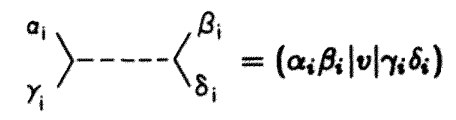
\includegraphics[width=6cm]{p1.png}
    \caption*{Fig.1}\label{}
\end{figure}
\begin{figure}[H]
    \centering
    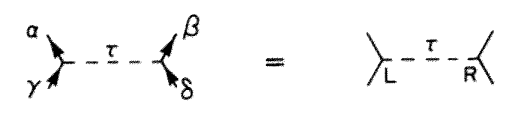
\includegraphics[width=6cm]{p2.png}
    \caption*{Fig.2}\label{}
\end{figure}
We derive the rules for constructing labeled diagrams which give a faithful 
representation of the complete set of contractions contributing to the $\rm n^{th}$ 
perturbation expansion of $\tiny \frac{Z}{Z_0}$.
\begin{itemize}
    \item Draw all distinct labeled diagrams composed of $n$ vertices connected 
    by directed lines. Two diagrams are distinct if they can't be deformed so as 
    to coincide completely, including all times labels $\tau_i$, left-right 
    labels $\rm L-R$ and the direction of arrows on propagators.
    \item assign a single-particle index to each directed line and include the 
    corresponding factor:
    \begin{figure}[H]
        \centering
        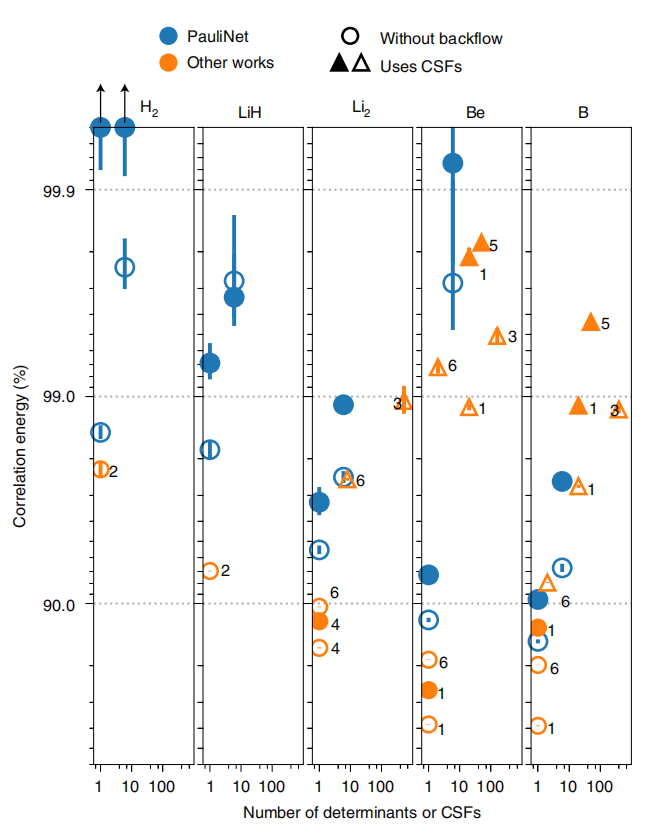
\includegraphics[width=15cm]{p3.png}
        \caption*{}
        \label{}
    \end{figure} 
    \item For each vertex, include the following factor:
    \begin{figure}[H]
        \centering
        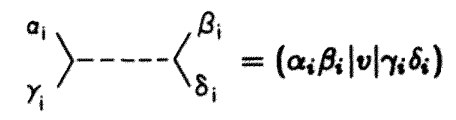
\includegraphics[width=6cm]{p1.png}
        \caption*{}
        \label{}
    \end{figure}
    \item Sum over all single-particle indices and integrate over all times over 
    the interval $[0,\beta]$.
    \item Multiply the result by the factor $\frac{(-1)^n}{n!2^n}\zeta^{n_L}$, 
    where $n_L$ is the number of closed loops in the diagram.
\end{itemize}
\subsection*{Labeled Feynman Diagrams} 
For a general interaction which has no special properties other than the symmetry
\begin{equation*}
    (\alpha\beta|v|\gamma\delta)=(\beta\alpha|v|\delta\gamma)
\end{equation*}
There are two types of transformations leaving the value of a diagram invariant. 
One is permutation of times labels $\tau_1\tau_2\dots\tau_n$, cause all times labels 
are integrated over $[0,\beta]$. the other is the exchange of extremities of each 
vertex, according to the symmetry of the interaction matrix.

The most general transformation leaving the value of a diagram invariant is the 
combination of a permutation of times labels and an exchange of vertex extremities. 
This kind of transformations of an $\rm n^{th}$ order diagram is a group, denoted by 
$G$. Consider the action of this group of transformations, $G$, on a labeled diagram 
$\Gamma$. Some set of transformations $G_{\Gamma}$ will transform $\Gamma$ into a 
deformation of itself, while the rest of transformations will yield diagrams which 
are distinct from $\Gamma$. $G_{\Gamma}$ defined in this way is a subgroup of $G$.

We define $S$ as the number of deformations of $\Gamma$ generated by the action of 
$G$. $S$ is the number of elements of $G_\Gamma$. since $G_\Gamma$ is a subgroup 
of $G$, $S$ is a divisor of $2^nn!$. consider a diagram $\Gamma'$ which is distinct 
from $gamma$ and is generated from $\Gamma$ by a transformation of $G$. Cause 
$\Gamma'$ corresponds to some permutation of $\tau$ and $\rm L-R$ lables on $\Gamma$, 
it transforms into deformation of itself under $G_\Gamma$. ($G$ is an Abelian group.) 
Thus $\Gamma'$ has $S$ deformations of itself. And the $2^nn!$ diagrams generated 
by action of $G$ on $\Gamma$ can be grouped into $\frac{2^nn!}{S}$ sets of $S$ 
diagrams, S.t. diagrams in the same set are deformation of each other and diagrams 
in different sets are distinct. All distinct diagrams will thus be counted correctly 
if we multiply the value of one diagram by the factor $\frac{2^nn!}{S}$.

An unlabeled diagram is obtained by removing times and $\rm L-R$ labels on vertices 
from a labeled diagram. It is composed of completely unlabeled vertices connected by 
directed lines. The rules of drawing the $\rm n^{th}$ order contribution to the 
perturbation expansion of $\tiny \frac{Z}{Z_0}$ are summarized.
\begin{itemize}
    \item Draw all distinct unlabeled diagrams composed of $n$ vertices connected by 
    directed lines. Two diagrams are distinct if they cannot be deformed so as to 
    coincide completely including the direction of arrows on propagators.
    \item Calculate the symmetry factor $S$ for the diagram.
    \item Assign a time label $\tau_i$ to each vertex, and a single-particle index 
    to each directed line. For each directed line include the factor.
    \begin{figure}[H]
        \centering
        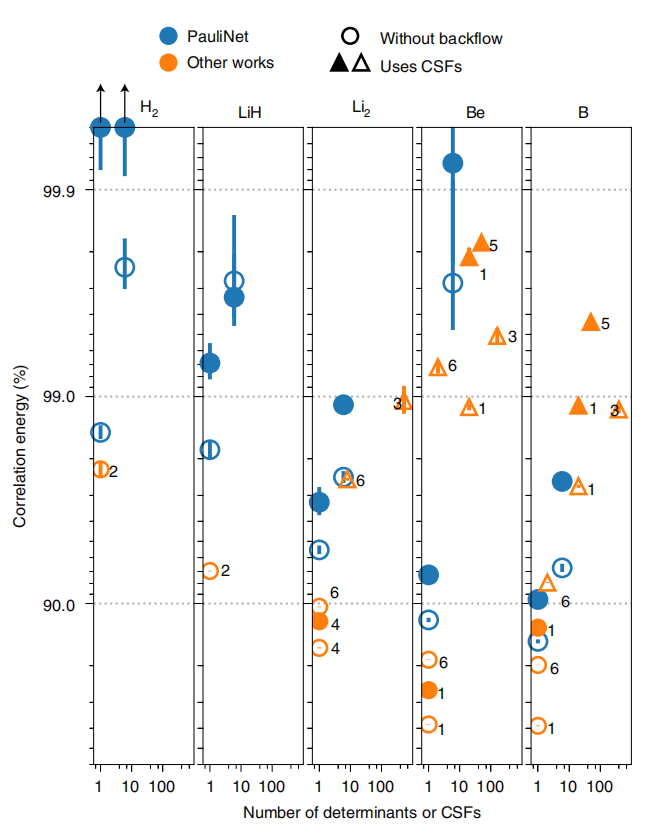
\includegraphics[width=15cm]{p3.png}
        \caption*{}
        \label{}
    \end{figure}
    \item For each vertex, include the factor
    \begin{figure}[H]
        \centering
        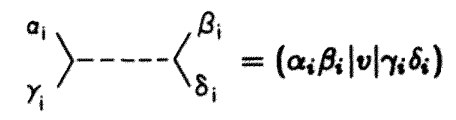
\includegraphics[width=6cm]{p1.png}
        \caption*{}
        \label{}
    \end{figure} 
    \item Sum over all single-particle index and integrate all times labels over the 
    interval $[0,\beta]$.
    \item Multiply the result by the factor $\frac{(-1)^n}{S}\zeta^{n_L}$. 
\end{itemize}
\begin{figure}[H]
    \centering
    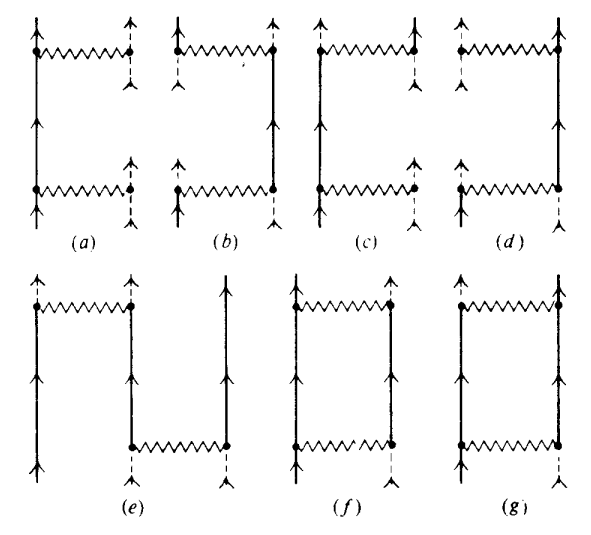
\includegraphics[width=13cm]{p4.png}
    \caption*{Fig.3  Second order unlabeled Feynman diagrams with symmetry factor 
    $\frac{1}{S}$}
    \label{}
\end{figure} 
If we regard the product of an interaction and two propagators as a matrix in the 
time and single-particle labels:
\begin{figure}[H]
    \centering
    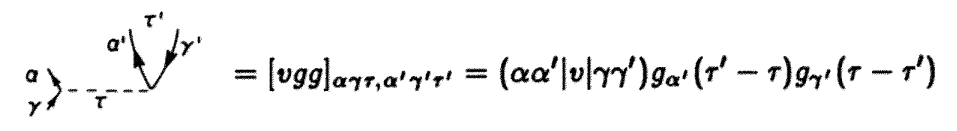
\includegraphics[width=15cm]{p5.png}
    \caption*{}
    \label{}
\end{figure}
Then the sum of first order diagrams and all direct ring diagrams is 
\begin{equation*}
    \sum_{n=1}^\infty\frac{(-\zeta)^n}{2n}\Tr[vgg]^n
\end{equation*}
that is 
\begin{figure}[H]
    \centering
    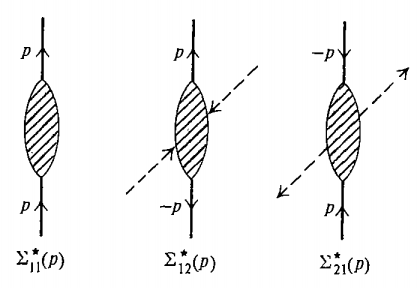
\includegraphics[width=8cm]{p6.png}
    \caption*{}
    \label{}
\end{figure}
In the $\rm n^{th}$ order contribution, there is totally $(2n)!$ labeled diagrams. And for 
each transformation group $G$, the number of distinct diagrams corresponding to a 
unlabeled diagram is $\frac{2^nn!}{S}$. Hence
\begin{equation*}
    \sum\frac{2^nn!}{S}=(2n)!
\end{equation*} 
\begin{equation*}
    \sum\frac{1}{S}=\frac{(2n)!}{2^nn!}=(2n-1)!!
\end{equation*} 
For the second order case, all the eight unlabeled diagrams and their symmetry 
factors are shown in Fig.(3). And it indeed satisfy the equation above.
\subsection*{Hugenholtz Diagrams}
For many purposes it is convenient to combine the unlabeled Feynman diagrams in a 
single symmetrized or antisymmetrized matrix element. The resulting diagram is 
called Hugenholtz diagram. We again consider the case of a two-body potential. 
Since we no longer wish to distinguish direct and exchange diagrams, the vertix 
will now be represented by a dot with two incoming and outgoing lines:
\begin{figure}[H]
    \centering
    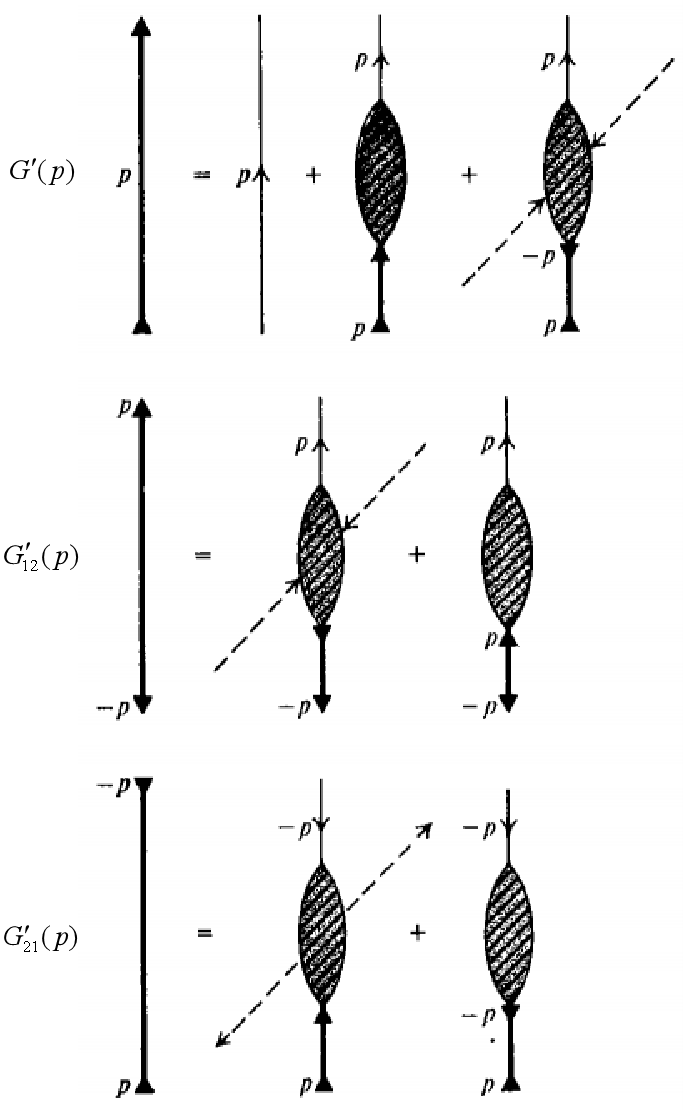
\includegraphics[width=5cm]{p7.png}
    \caption*{}
    \label{}
\end{figure}
The rules for calculating $\rm n^{th}$ order contribution to the pertubation expansion 
of $\tiny \frac{Z}{Z_0}$ using Hugenholtz diagrams:
\begin{itemize}
    \item Draw all distinct labeled diagrams composed of $n$ vertices connected 
    by directed lines. Two diagrams are distinct if they can't be deformed so as 
    to coincide completely, including the direction of arrows on propagators.
    \item Calculate the symmetry factor $S$ for the diagram. Add times labels to each 
    vertex, and $S$ is the number of time permutations which transform the diagrams 
    to a deformation of itself.
    \item Assign a time label $\tau_i$ to each vertex and a single-particle index to 
    each directed line. For each directed line include the factor:
    \begin{figure}[H]
        \centering
        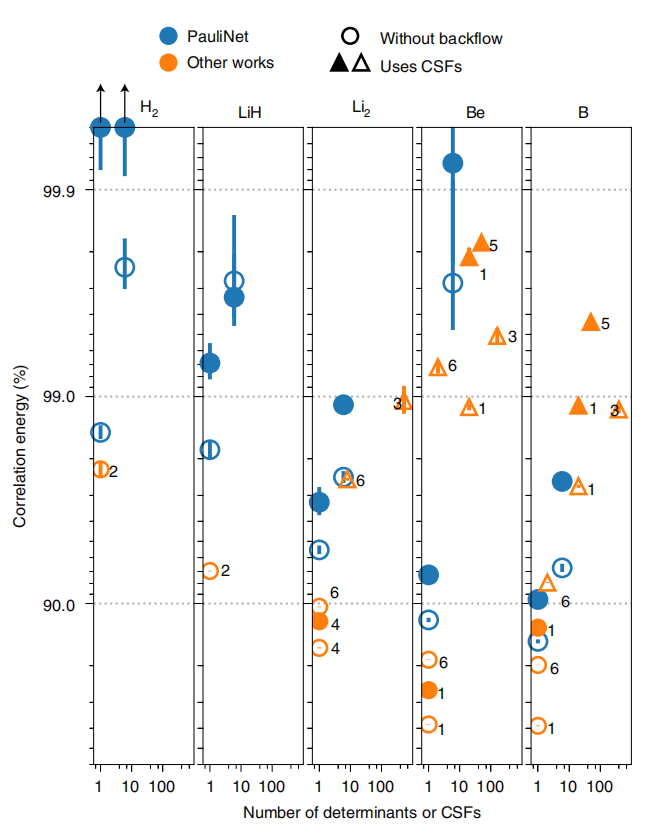
\includegraphics[width=15cm]{p3.png}
        \caption*{}
        \label{}
    \end{figure}
    \item For each vertex, include the factor:
    \begin{figure}[H]
        \centering
        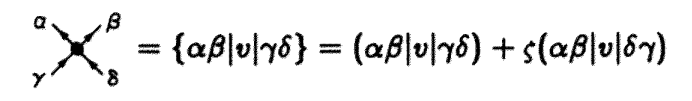
\includegraphics[width=10cm]{p10.png}
        \caption*{}
        \label{}
    \end{figure}
    \item Sum over all single-particle index and integrate all times over the 
    interval $[0,\beta]$
    \item Multiply the result by the factor $\frac{(-1)^n\zeta^{n_L}}{2^{n_e}S}$,
    where $n_e$ is the number of pairs of lines begining at the same vertex,  
    terminating at the same end, and oriented in the same direction. 
\end{itemize}

\begin{figure}[H]
    \centering
    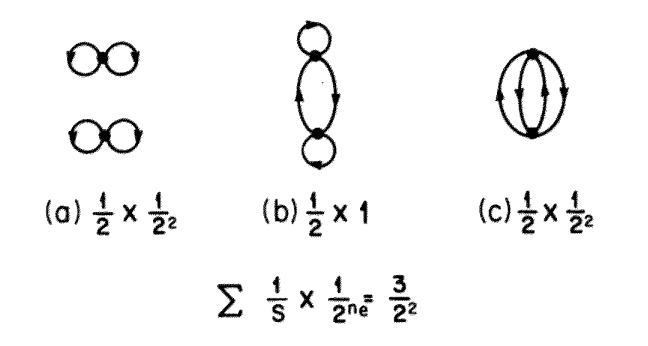
\includegraphics[width=12cm]{p8.png}
    \caption*{Fig.4 Second order Hugenholtz diagrams with symmetry factors}
    \label{}
\end{figure}
\begin{figure}[H]
    \centering
    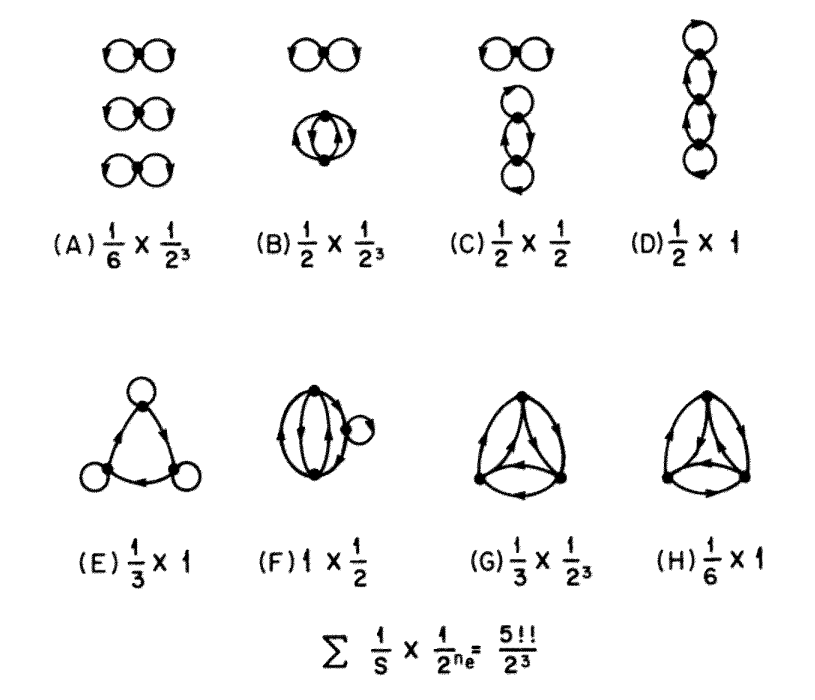
\includegraphics[width=12cm]{p9.png}
    \caption*{Fig.5 Third order Hugenholtz diagrams with symmetry factors}
    \label{}
\end{figure}
\subsection*{Frequency and Momentum Representation}
For problems which are homogeneous in time, it is useful to Fourier transform from 
time to frequency.

For a function of time $g(\tau)$ which is periodic or antiperiodic in the interval 
$[0,\beta]$, we write the Fourier series as:
\begin{equation*}
    \begin{split}
        \tilde{g}(\omega_n)=\int_0^\beta d\tau e^{i\omega_n\tau}g(\tau)\\
        g(\tau)=\frac{1}{\beta}\sum_{\omega_n}e^{-i\omega_n\tau}\tilde{g}(\omega_n)
    \end{split}
\end{equation*}
Where for the periodic functions
\begin{equation*}
    \omega_n=\frac{2n\pi}{\beta}
\end{equation*}
while for the antiperiodic functions
\begin{equation*}
    \omega_n=\frac{2(n+1)\pi}{\beta}
\end{equation*}
Denoting the discrete momentum $\vec{k}_n\equiv(k^x_{n_x},k^y_{n_y},k^z_{n_z})$, and 
the volume $\mathcal{V}=L_xL_yL_z$. The matrix element of potential $v$ evaluated 
with the normalized eigenstates is:
\begin{equation*}
    \begin{split}
        (\vec{k}_{n_1}\vec{k}_{n_2}|v|\vec{k}_{n_3}\vec{k}_{n_4})&=\int
        \frac{d^3x_1d^3x_2}{\mathcal{V}^2}v(\vec{x}_1-\vec{x}_2)e^{i
        [(\vec{k}_1-\vec{k}_3)\cdot\vec{x}_1+(\vec{k}_2-\vec{k}_4)\cdot\vec{x}_2]}\\
        &=\int\frac{d^3rd^3R}{\mathcal{V}^2}v(\vec{r})e^{i\vec{R}(\vec{k}_{n_1}
        +\vec{k}_{n_2}-\vec{k}_{n_3}-\vec{k}_{n_4})+\frac{i\vec{r}}{2}(\vec{k}_{n_1}
        -\vec{k}_{n_3}+\vec{k}_{n_4}-\vec{k}_{n_2})}\\
        &=\frac{1}{\mathcal{V}}\delta_{\vec{k}_{n_1}+\vec{k}_{n_2},\vec{k}_{n_3}+
        \vec{k}_{n_4}}v(\vec{k}_{n_1}-\vec{k}_{n_3})
    \end{split}
\end{equation*} 
Thus, each interaction conserves momentum. Every diagram can be decomposed into 
several connected parts. In fig.5, diagram A has three connected parts, diagrams B 
and C have two connected parts and diagrams D through H has only one connected part.

Fourier transformation from $\tau$ to $\omega$ for a problem which is homogeneous in 
time: (notice that $\omega=\frac{2n\pi}{\beta}$ for Bosons and 
$\omega=\frac{(2n+1)\pi}{\beta}$ for Fermions, and $e^{i\beta\omega_n}=\zeta$.)
\begin{equation*}
    \begin{split}
        \tilde{g}_\alpha&=\int_0^\beta d\tau e^{(i\omega_n-(\epsilon_\alpha-\mu))\tau}
        [\theta(\tau)(1+\zeta n_\alpha)+\zeta\theta(-\tau)n_\alpha]\\
        &=\int_0^\beta d\tau e^{(i\omega_n-(\epsilon_\alpha-\mu))\tau}(1+\zeta n_\alpha)\\
    \end{split}
\end{equation*}
Notice that
\begin{equation*}
    n_\alpha=\frac{1}{e^{\beta(\epsilon_\alpha-\mu)-\zeta}}
\end{equation*}
thus we obtain:
\begin{equation*}
    \begin{split}
        \tilde{g}_\alpha&=\frac{\zeta e^{\beta(\epsilon_\alpha-\mu)}-1}
        {i\omega_n-(\epsilon_\alpha-\mu)}\frac{e^{\beta(\epsilon_\alpha-\mu)}}
        {e^{\beta(\epsilon_\alpha-\mu)}-\zeta}\\
        &=\frac{\zeta-e^{\beta(\epsilon_\alpha-\mu)}}{[i\omega_n-(\epsilon_\alpha-\mu)]
        (e^{\beta(\epsilon_\alpha-\mu)}-\zeta)}\\
        &=-\frac{1}{i\omega_n-(\epsilon_\alpha-\mu)}
    \end{split}
\end{equation*}
And hence
\begin{equation*}
    g_\alpha(\tau)=-\sum_{\omega_n}\frac{1}{\beta}e^{-i\omega_n\tau}
    \frac{1}{i\omega_n-(\epsilon_\alpha-\mu)}
\end{equation*}
In order to invoke the proper $\theta$-function in the case where the propagator 
begins and ends at the same vertex, the argument is always shifted by an infinitesimal 
$\eta$ to $g_\alpha(\tau-\eta)$. This same result may be obtained by multiplying 
$\tilde{g}_\alpha(\omega_n)$ by the factor $e^{i\omega_n\eta}$, in which case:
\begin{equation*}
    \begin{split}
        \frac{1}{\beta}\sum_{\omega_n}e^{-i\omega_n(\tau-\eta)}\tilde{g}_\alpha(\omega_n)
        &=-\frac{1}{\beta}\sum_{\omega_n}e^{-i\omega_n(\tau-\eta)}
        \frac{1}{i\omega_n-(\epsilon_\alpha-\mu)}\\
        &=g_\alpha(\tau-\eta)
    \end{split}
\end{equation*} 
Acoording to calculation, the contribution of an $\rm n^{th}$ order diagram is 
proportional to $\beta^{-n}$, then the diagram rules presented previously are 
modified as follows in frequency representation.
\begin{itemize}
    \item Assign frequency labels to each directed line as follows. Within each 
    each connected part containing $m$ interactions, select $m+1$ propagators to 
    label independently and use frequency conservation at each vertex to label 
    remaining propagators. Assign single-particle indices as before. For each 
    directed line include the factor:
    \begin{figure}[H]
        \centering
        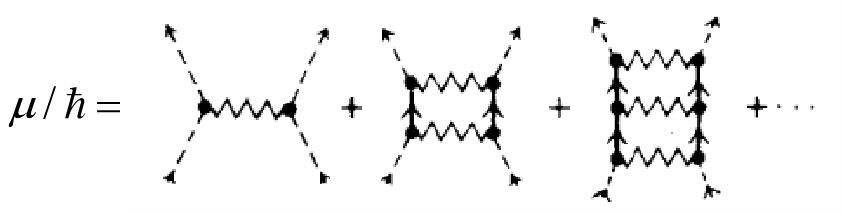
\includegraphics[width=8cm]{p11.png}
        \caption{}
        \label{}
    \end{figure} 
    For propagators begining and ending at the same vertex, include an additional 
    factor $e^{i\omega_n\eta}$.
    \item Sum over all single-particle indices, and sum over all frequencies 
    $\omega_n$.
    \item Multiply the factor defined previously by $\frac{1}{\beta^m}$, where 
    $m$ is the number of interactions.

    The generalization of these rules using momentum and frequency representation 
    to n-body interacions is straightforward. It is often convenient to use 
    momentum and frequency representation simultaneously in which case one 
    associates with each propagator with a four-momentum $(\omega_n,k)$, which is 
    conversed at each vertex.
\end{itemize} 

The expansion of $Z$ contains all power of the volume $\mathcal{V}$, with an 
individual diagram with $n_c$ connected parts being proportional to 
$\mathcal{V}^{n_c}$. Thus it is not an extensive quantity. In contrast, the 
ground potential $\Omega=-\frac{1}{\beta}\ln Z=-P\mathcal{V}$ is an extensive 
quantity. So it must be possible to find an extensive expansion of $\Omega$.
The linked cluster theorem states that $\ln Z$ is in fact given by the sum of all  
connected diagrams.

We will derive this theorem using replica technique. The basic idea of replica 
method is to evaluate $Z^n$ for integer $n$ by replicating the system $n$ 
times and expand the result as follows:
\begin{equation*}
    Z^n=e^{n\ln Z}=1+n\ln Z+\sum_{m=2}^\infty\frac{(n\ln Z)^m}{m!}
\end{equation*} 
in which $\ln Z$ is given by the coefficients of terms proportional to $n$. 
A more general statement of this method is to calculate $Z^n$, and continue 
the function to $n=0$:
\begin{equation*}
    \begin{split}
        \lim_{n\rightarrow0}\frac{d}{dn}Z^n&=\lim_{n\rightarrow0}\frac{d}{dn}
        (e^{n\ln Z})\\
        &=\ln Z
    \end{split}
\end{equation*}
We first evaluate $Z^n$ for integer $n$ by perturbation. $\ln Z$ will be given 
by the coefficient of graphs proportional to $n$. Remember that
\begin{equation*}
    Z=\int\limits_{\psi_\alpha(\beta)=\zeta\psi_\alpha(0)}\mathcal{D}
    (\psi^*_\alpha(\tau),\psi_\alpha(\tau))e^{-\int_0^\beta d\tau[\sum_\alpha
    \psi^*_\alpha(\tau)(\partial_\tau+\epsilon_\alpha-\mu)\psi_\alpha(\tau)+
    V(\psi^*_\alpha(\tau),\psi_\alpha(\tau))]}
\end{equation*}
We may write $Z^n$ as a function integral over $n$ sets of fields 
${\psi^{\sigma*}_\alpha(\tau),\psi^\sigma_\alpha(\tau)}$
\begin{equation*}
    \begin{split}
        (\frac{Z}{Z_0})^n&=\frac{1}{Z_0^n}\int\limits_{\psi^\sigma_\alpha(\beta)
        =\zeta\psi^\sigma_\alpha(0)}\prod_{\sigma=1}^n\mathcal{D}
        (\psi^{\sigma*}_\alpha(\tau),\psi^\sigma_\alpha(\tau))\\
        &\times e^{-\int\limits_0^\beta d\tau\sum_{\sigma=1}^n[\sum_\alpha\psi^{\sigma*}
        _\alpha(\tau)(\partial_\tau+\epsilon_\alpha-\mu)\psi^\sigma_\alpha(\tau)
        +V(\psi^{\sigma*}_\alpha,\psi^\sigma_\alpha)]}
    \end{split}
\end{equation*}
Now, all propagators leaving or entering a given vertex have the same index 
$\sigma$, and all $\sigma$'s are summed from $1$ t0 $n$. It is evident that 
each connected part of a diagram must carry a single index $\sigma$, which when 
summed from $1$ to $n$, yields a factor $n$. Thus, a graph with $n_c$ connected 
parts is proportional to $n_c$ and graphs proportional to $n$ are those with 
only one connected part, that is connected graphs. As a consequence, we obtain 
the linked cluster theorem:
\begin{equation*}
    \Omega-\Omega_0=\frac{1}{\beta}\sum(\rm all\ connected\ graphs)
\end{equation*} 
Where $\Omega_0$ is the grand potential of the unperturbed system
\begin{equation*}
    \Omega_0=\frac{\zeta}{\beta}\sum_\alpha\ln(1-\zeta e^{-\beta(\epsilon_\alpha
    -\mu)})
\end{equation*}
\subsection*{Calculations Of Observables And Greens Function}
The expectation value of operator $R$ can be written as
\begin{equation*}
    \begin{split}
        \langle R\rangle&=\frac{\int\mathcal{D}(\psi^*_\alpha,\psi_\alpha)
        \Big[e^{-\int\limits_0^\beta d\tau\sum_\alpha\psi^*_\alpha(\partial_\tau+
        \epsilon_\alpha-\mu)\psi_\alpha+V(\psi^*_\alpha,\psi_\alpha)}
        R(\psi^*_\alpha(0),\psi_\alpha(0))\Big]}{\int\mathcal{D}(\psi^*_\alpha,
        \psi_\alpha)e^{-\int\limits_0^\beta d\tau\sum_\alpha\psi^*_\alpha(\partial_\tau
        +\epsilon_\alpha-\mu)\psi_\alpha+V(\psi^*_\alpha,\psi_\alpha)}}\\
        &=\frac{\Big\langle e^{-\int\limits_0^\beta d\tau V(\psi^*_\alpha,
        \psi_\alpha)}R(\psi^*_\alpha(0),\psi_\alpha(0))\Big\rangle_0}
        {\Big\langle e^{-\int\limits_0^\beta d\tau V(\psi^*_\alpha,\psi_\alpha)}
        \Big\rangle_0}
    \end{split}
\end{equation*}
Use the replica technique again. introduce n fields ${\psi^{\sigma*}_\alpha,
\psi^\sigma_\alpha}$ where $\sigma$ runs from $1$ to $n$
\begin{equation*}
    \begin{split}
        R_n&=Z_0^{-n}\int\mathcal{D}(\psi^{\sigma*}_\alpha,\psi^\sigma_\alpha)
        R(\psi^{1*}_\alpha(0),\psi^1_\alpha(0))\\
        &\times e^{-\int\limits_0^\beta d\tau\sum_{\sigma=1}^n[
            V(\psi^{\sigma*}_\alpha,psi^\sigma_\alpha)+\sum_\alpha\psi^{\alpha*}
            _\alpha(\partial_\tau+\epsilon_\alpha-\mu)\psi^\sigma_\alpha]}
    \end{split}
\end{equation*}
Note that the operator $R$ is calculated with the field $\psi^{1*}_\alpha,
\psi^1_\alpha$ associated with $\sigma=1$ and is evaluated at $\tau=0$. By 
seperating the $\sigma=1$ component from the $n-1$ other components, we obtain
\begin{equation*}
    R_n=\Big\langle e^{-\int\limits_0^\beta d\tau V(\psi^*_\alpha,\psi_\alpha)}
    R(\psi^*_\alpha(0),\psi_\alpha(0))\Big\rangle_0\Big\langle e^{-\int\limits_0
    ^\beta d\tau V(\psi^*_\alpha,\psi_\alpha)}\Big\rangle_0^{n-1}
\end{equation*}
thus the expectation value of $R$ is obtained when $n=0$:
\begin{equation*}
    \langle R\rangle=R_0
\end{equation*}  
The perturbation expansion of $R_n$ is 
\begin{equation*}
    \begin{split}
        R_n&=\sum_{m=0}^\infty\frac{(-1)^m}{m!}\sum_{\sigma_1=1}^n\dots
        \sum_{\sigma_m=1}^n\int_0^\beta d\tau_1\dots d\tau_m\\
        &\times\langle V(\psi^{*\sigma_1}_\alpha(\tau_1),\psi^{\sigma_1}_\alpha(\tau_1))
        \dots V(\psi^{*\sigma_p}_\alpha(\tau_p),\psi^{\sigma_p}_\alpha(\tau_p))
        R(\psi^{*1}_\alpha(0),\psi^1_\alpha(0))\rangle_0
    \end{split}
\end{equation*}
Since $R$ is constrained to carry $\sigma=1$, $\sigma$ must be $1$ everywhere 
in the portion of the diagram linked to $R$. In the additional disconnected 
parts, there is at least one summation over $\sigma$ leadind to an overall 
factor of at least one power of $n$. Hence all diagrams with disconnected parts 
will vanish when $n$ is set equal to $0$, and $\langle R\rangle$ is given by all 
connected diagrams linked to $R$.

The symmetry factor $S$ of such diagrams containing an operator labeled $R$ is 
$1$ or $2$. Only $S$ of a diagram which are symmetric on both side of $R$ is 
$2$, in which case a permutation of times $\tau_i$ perform a deformation of 
the diagram. Thus we can summarize the rules for calculating the $p^{\rm th}$ 
order contribution to the perturbation expansion of the expectation value of a 
two-body operator $\langle R\rangle$ using unlabeled Feynman diagrams:
\begin{itemize}
    \item Draw all distinct unlabeled connected diagrams composed of one 
    $R$-vertex and $p$ $v$-vertices connected by directed lines. Two diagrams 
    are distinct if they can't be deformed so as to coincide completely 
    including the directions on propagators. For each distinct diagram, 
    evaluate the contribution as follows.
    \item Calculate the symmetry factor $S$ for the diagram. If the exchange 
    of the extremities of $R$ with some permutations of times and exchanges 
    of extremities of interactions yields a deformation of itself, $S=2$. 
    Otherwise, $S=1$.
    \item Assign a time label $\tau_i$ to each $v$-vertex, associate $\tau=0$ 
    with the $R$-vertex, and assign a single-particle index to each directed 
    line. For each directed line include the factor:
    \begin{figure}[H]
        \centering
        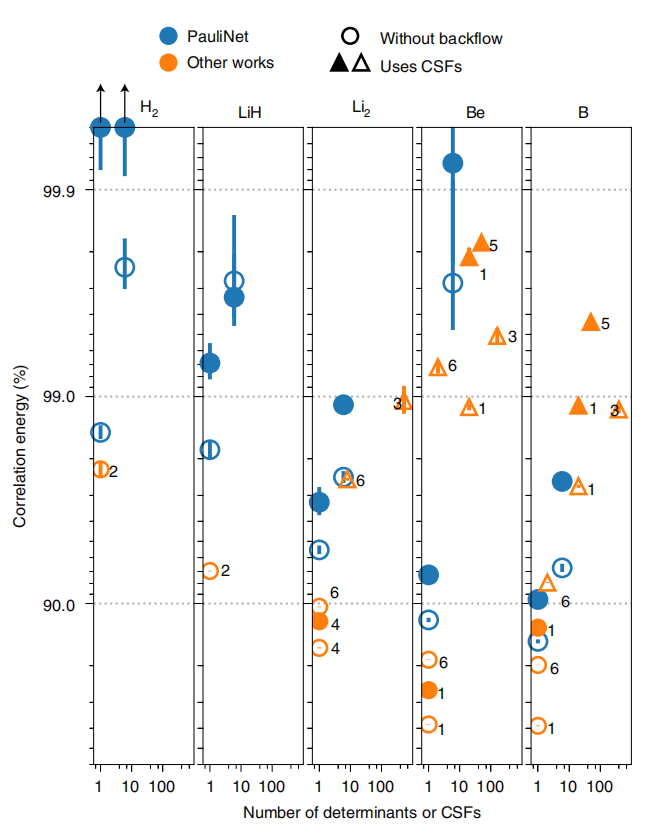
\includegraphics[width=15cm]{p3.png}
        \caption*{}
        \label{}
    \end{figure}
    \item For each $v$-vertex include the factor 
    \begin{figure}[H]
        \centering
        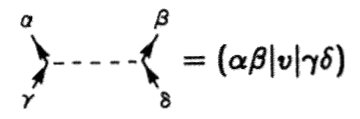
\includegraphics[width=5cm]{p12.png}
        \label{}
    \end{figure}
    \item For each $R$-vertex include the factor
    \begin{figure}[H]
        \centering
        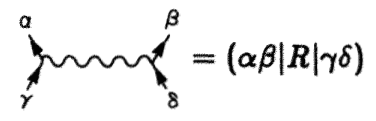
\includegraphics[width=5cm]{p13.png}
        \label{}
    \end{figure}
    \item Sum over all single-particle indices and integrate $p$ times over 
    the interval $[0,\beta]$.
    \item Multiply the result by the factor $\frac{(-1)^p}{S}\zeta^{n_L}$, where 
    $n_L$ is the number of closed loops and $S$ is the symmetry number. 
\end{itemize} 
\begin{figure}[H]
    \centering
    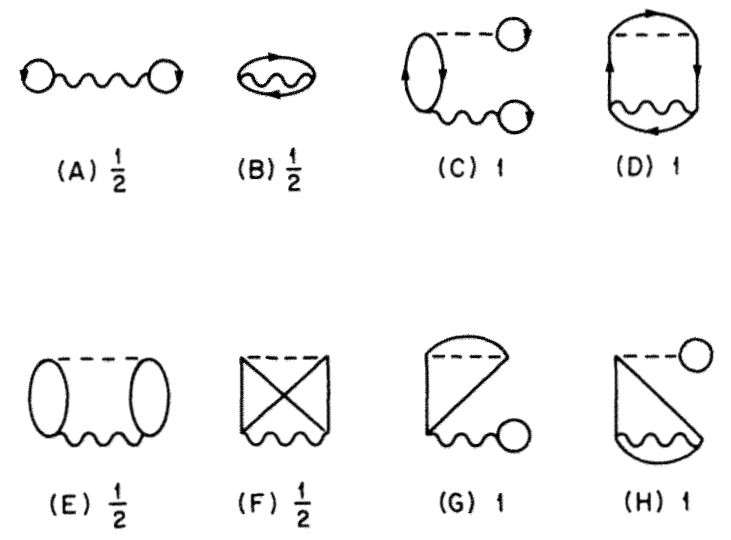
\includegraphics[width=12cm]{p14.png}
    \caption*{Fig.6 Unlabeled Feynman diagrams for $\langle R\rangle$ with 
    factor $\frac{1}{S}$}
    \label{}
\end{figure}
The eight unlabeled diagrams contributing to $\langle R\rangle$ in orders $p=0$ 
and $p=1$ are shown in Fig.6, together with the factors $\frac{1}{S}$. The 
contribution at order $0$ is given by diagrams A and B. 
\begin{equation*}
    \langle R\rangle^{(0)}=\frac{1}{2}\sum_{\alpha,\beta}[(\alpha\beta|R|
    \alpha\beta)+\zeta(\alpha\beta|R|\beta\alpha)]n_\alpha n_\beta
\end{equation*}
and a typical contribution at order $1$ is that of diagram E
\begin{equation*}
    \langle R\rangle^{(E)}=-\frac{1}{2}\sum_{\alpha\beta\gamma\delta}
    \int_0^\beta d\tau(\alpha\beta|R|\gamma\delta)(\gamma\delta|v|\alpha\beta)
    g_\alpha(-\tau)g_\beta(-\tau)g_\gamma(\tau)g_\delta(\tau)
\end{equation*}
The derivation of the diagrammatic expansion for the imaginary-time Green's 
function 
\begin{equation*}
    \begin{split}
        &\mathcal{G}^{(n)}(\alpha_1\beta_1,\dots\alpha_n\beta_n|\alpha'_1\beta'_1,
        \dots\alpha'_n\beta'_n)\\
        &=\frac{\langle e^{-\int d\tau V(\psi_\alpha^*(\tau),
        \psi_\alpha(\tau))}\psi_{\alpha_1}(\beta_1)\dots\psi_{\alpha_n}(\beta_n)
        \psi^*_{\alpha'_n}(\beta'_n)\dots\psi^*_{\alpha'_1}(\beta'_1)\rangle_0}
        {\langle e^{-\int d\tau V(\psi_\alpha^*(\tau),\psi_\alpha(\tau))}\rangle_0}
    \end{split}
\end{equation*}
is analogous to that for the expectation value $\langle R\rangle$ with the 
operator $R(\psi^*_\alpha(0),\psi_\alpha(0))$ replaced by $\psi_{\alpha_1}
(\beta_1)\dots\psi_{\alpha_n}(\beta_n)\psi^*_{\alpha'_n}(\beta'_n)\dots
\psi^*_{\alpha'_1}(\beta'_1)$. The symmetry factor of a Green's function is 
$1$. The rules for calculating the $\rm r^{th}$ order contribution to the 
expansion of Green's function $\mathcal{G}^{(n)}(\alpha_1\beta_1,\dots
\alpha_n\beta_n|\alpha'_1\beta'_1,\dots\alpha'_n\beta'_n)$ using unlabeld 
Feynman diagrams are as follows:
\begin{itemize}
    \item Draw all distinct unlabeled connected diagrams composed of n external 
    points $\psi_{\alpha_i}(\beta_i)$, n external points $\psi^*_{\alpha'_i}
    (\beta'_i)$, and $r$ interaction vertices connected by directed lines.
    \item Each external point correspond to a specified state $\alpha_i$ and 
    time $\beta_i$. Assign a internal time label $\tau_i$ to each of the $r$ 
    interaction vertices and for any propagator which is not connected to an 
    external point assign an internal single-particle index. For each directed 
    line include the factor
    \begin{figure}[H]
        \centering
        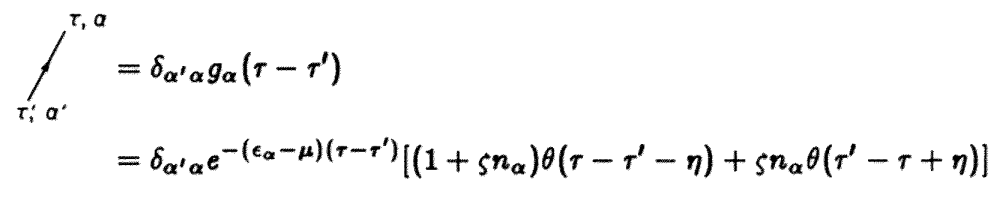
\includegraphics[width=15cm]{p15.png}
        \label{}
    \end{figure}
    \item For each interaction vertex include the factor
    \begin{figure}[H]
        \centering
        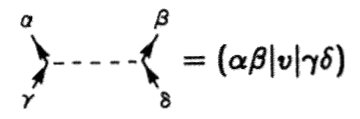
\includegraphics[width=5cm]{p12.png}
        \label{}
    \end{figure}
    \item Sum over all single-particle indices and integrate $r$ times $\tau_i$ 
    over the interval $[0,\beta]$.
    \item Multiply the result by the factor $(-1)^r\zeta^{P}\zeta^{n_L}$ where 
    $n_L$ is the number of closed loops and $\zeta^P$ is the sign of the 
    permutation $P$ such that each propagator line originating at the external 
    point $\psi^*_{\alpha'_m}(\beta'_m)$ terminates at the external point 
    $\psi^*_{\alpha_{Pm}}(\beta_{Pm})$
\end{itemize}
\begin{figure}[H]
    \centering
    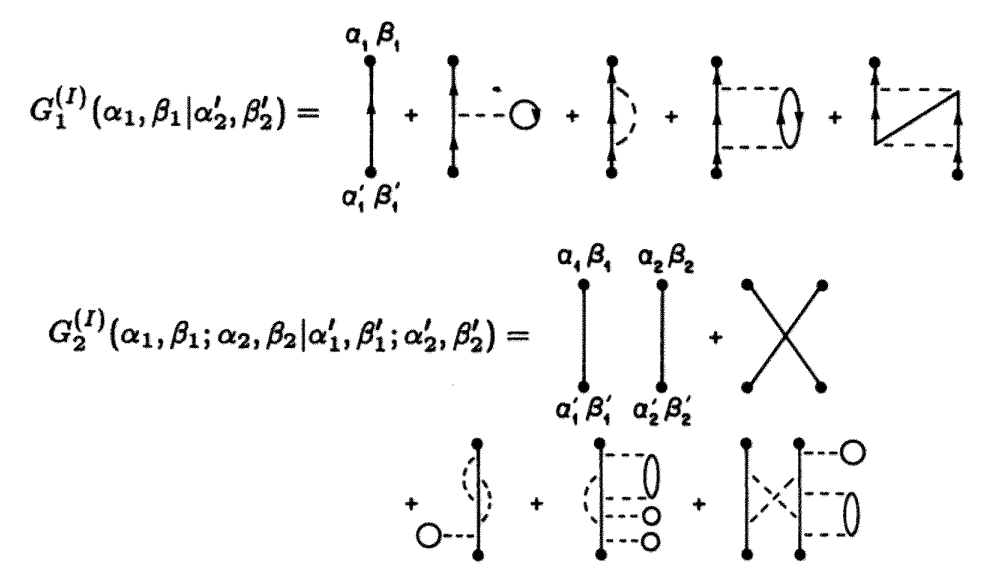
\includegraphics[width=12cm]{p16.png}
    \caption*{Fig.7 Diagrams contributing to one- and two-particle Green's 
    functions with overall sign factors.}
    \label{}
\end{figure}
Examples of graphs of contributing to the one- and two-particle Green's 
functions, together with the overall sign factor are given in Fig.(7)
\subsection*{The Effective Potential}
In the presence of soources, the operators $\{a^\dagger_\alpha(\tau),a_\alpha
(\tau)\}$ acquire non-zero expectation values. We define the average field
\begin{equation*}
    \begin{split}
        \phi_\alpha&=\langle a_\alpha\rangle_{J^*,J}=\langle \psi_\alpha
        \rangle_{J^*,J}\\
        &=\frac{\int\mathcal{D}[\psi^*_\alpha\psi_\alpha]\psi_\alpha
        e^{-\int\limits_0^\beta d\tau\left[\sum_\alpha\psi^*_\alpha(\partial_\tau
        -\mu)\psi_\alpha+H[\psi^*_\alpha\psi_\alpha]+\sum_\alpha[J^*_\alpha
        \psi_\alpha+\psi^*_\alpha J_\alpha]\right]}}{\int\mathcal{D}[\psi^*_\alpha
        \psi_\alpha]e^{-\int\limits_0^\beta d\tau\left[\sum_\alpha\psi^*_\alpha
        (\partial_\tau-\mu)\psi_\alpha+H[\psi^*_\alpha\psi_\alpha]+\sum_\alpha
        [J^*_\alpha\psi_\alpha+\psi^*_\alpha J_\alpha]\right]}}\\
        &=-\frac{\delta}{\delta J^*_\alpha(\tau)}W[J^*_\alpha(\tau),J_\alpha(\tau)]
    \end{split}
\end{equation*}
and its complex conjugate field
\begin{equation*}
    \begin{split}
        \phi^*_\alpha(\tau)&=\langle a^\dagger_\alpha(\tau)\rangle_{J^*,J}\\
        &=-\zeta\frac{\delta}{\delta J_\alpha(\tau)}W[J^*_\alpha(\tau),J_\alpha
        (\tau)]
    \end{split}
\end{equation*}
$\langle\ \ \ \rangle_{J^*,J}$ denotes a thermal average with respect to $H$ 
plus the sourse term.
Instead of dealing with the generating function $W$ as a function of the sources 
$J^*$, $J$, it is useful to perform a Legendre transformation to obtain a function 
of the fields $\phi^*$, $\phi$. Consider a familiar example of a spin system in 
a magnetic field. Denoting the Hamiltonian of the spin variable as 
$\mathcal{H}(s)$, the free energy as a function of an external magnetic field 
$\vec{H}$ is given by
\begin{equation*}
    \Tr e^{-\beta(\mathcal{H}(s)-\vec{H}\cdot\sum_i\vec{s}_i)}=e^{-\beta F(H)}
\end{equation*}
From which it follows that the magnetization is given by 
\begin{equation}
    M=-\frac{\partial F(H)}{\partial H}
\end{equation}
A state function which depends upon the magnetization instead of external 
magnetic field is obtained by inverting the relation (5) to obtain $H(M)$ and 
defining the Legendre transform
\begin{equation*}
    G(M)=F(H(M))+MH(M)
\end{equation*}
it follows that $G$ satisfies the reciprocity relation
\begin{equation*}
    \frac{\partial G}{\partial M}=\frac{\partial F}{\partial H}\frac{\partial H}
    {\partial M}+H+M\frac{\partial H}{\partial M}=H
\end{equation*}
Whereas both $F(H)$ and $G(M)$ contain the same physical information.

In the case of the generating function $W[J^*_\alpha(\tau),J_\alpha(\tau)]$, 
the equations for $\phi_\alpha(J^*_\alpha,J_\alpha)$ and $\phi_\alpha^*
(J^*_\alpha,J_\alpha)$ are inverted to obtain the sources as functions of the 
fields $J^*_\alpha(\phi^*_\alpha,\phi_\alpha)$ and $J_\alpha(\phi^*_\alpha,
\phi_\alpha)$ and the effective potential (effective action) is defined as the 
Legendre transform
\begin{equation*}
    \Gamma[\phi^*_\alpha(\tau),\phi_\alpha(\tau)]=-W[J^*_\alpha(\tau),
    J_\alpha(\tau)]-\sum_\gamma\int_0^\beta d\tau'[\phi^*_\gamma(\tau')J_\gamma
    (\tau')+J^*_\gamma(\tau')\phi_\gamma(\tau')]
\end{equation*}
As in the example $G(M)$, the effective potential satisfies the reciprocity 
relation
\begin{equation*}
    \begin{split}
        \frac{\partial}{\partial\phi^*_\alpha(\tau)}\Gamma[\phi^*_\alpha(\tau),
        \phi_\alpha(\tau)]&=-\sum_\gamma\int_0^\beta d\tau'\bigg[\frac{\partial
        W}{\partial J^*_\gamma(\tau')}\frac{\partial J^*_\gamma(\tau')}
        {\partial\phi^*_\alpha(\tau)}+\frac{\partial W}{\partial J_\gamma(\tau')}
        \frac{\partial J_\gamma(\tau')}{\partial\phi^*_\alpha(\tau)}\\
        &+\delta_{\gamma\alpha}\delta(\tau-\tau')J_\gamma(\tau')+\zeta
        \phi_\gamma^*(\tau')\frac{\partial J_\gamma(\tau')}{\partial\phi^*
        _\alpha(\tau)}+\frac{\partial J_\gamma^*(\tau')}{\partial\phi^*_\alpha
        (\tau)\phi_\gamma(\tau')}\bigg]\\
        &=-J_\alpha(\tau)
    \end{split}
\end{equation*}
and the companion equation
\begin{equation*}
    \frac{\partial}{\partial\phi_\alpha(\tau)}\Gamma[\phi^*_\alpha(\tau),
    \phi_\alpha(\tau)]=-\zeta J^*_\alpha(\tau)
\end{equation*}
When the sources are set equal to zero, the effective potential is stationary
\begin{equation*}
    \frac{\delta\Gamma(\tilde{\phi}^*_\alpha(\tau),\tilde{\phi}_\alpha(\tau))}
    {\delta\tilde{\phi}^*_\alpha(\tau)}=
    \frac{\delta\Gamma(\tilde{\phi}^*_\alpha(\tau),\tilde{\phi}_\alpha(\tau))}
    {\delta\tilde{\phi}_\alpha(\tau)}=0
\end{equation*}
Where $\tilde{\phi}^*_\alpha(\tau)$ and $\tilde{\phi}_\alpha(\tau)$ are denoted 
for the fields in the absence of sources. The effective potential is a 
generating function for vertex functions. Vertex functions are generated by 
differentiating the effective potential $\Gamma[\phi^*_\alpha(\tau)\phi
_\alpha(\tau)]$ just as connected Green's functions generated from $W$:
\begin{equation*}
    \begin{split}
        \Gamma_{m\phi^*,n\phi}&(\alpha_1\tau_1,\dots\alpha_m\tau_m|\alpha'_1
        \tau'_1,\dots\alpha'_n\tau'_n)\\
        &=\frac{\delta^{m=n}}{\delta\phi^*_{\alpha_1}(\tau_1)\dots\delta\phi^*
        _{\alpha_m}(\tau_m)\delta\phi_{\alpha'_n}(\tau'_n)\dots\delta\phi_
        {\alpha'_1}(\tau'_1)}\Gamma[\phi^*_\alpha(\tau),\phi_\alpha(\tau)]
        \Bigg|_{J^*_\alpha=J_\alpha=0}
    \end{split}
\end{equation*}
Note that evaluate at $J^*_\alpha=J_\alpha=0$ is equivalent to evaluation at 
the stationary solutions ${\tilde{\phi}^*_\alpha,\tilde{\phi}_\alpha}$.
\subsection*{The Self-energy And Dyson's Equation}
Before proceeding to the general case, it is useful to study the vertex 
function $\Gamma_{\phi^*\phi}$. The derivatives of a function $F$ can be 
written
\begin{equation*}
    \begin{split}
        \frac{\delta F(J^*,J)}{\delta\phi_{\alpha_1}(\tau_1)}&=\sum_{\alpha_2}
        \int\limits_0^\beta d\tau_2\Bigg[\frac{\delta F}{\delta J^*_{\alpha_2}
        (\tau_2)}\frac{\delta J^*_{\alpha_2}(\tau_2)}{\delta\phi_{\alpha_1}
        (\tau_1)}+\frac{\delta F}{\delta J_{\alpha_2}(\tau_2)}\frac{\delta 
        J_{\alpha_2}(\tau_2)}{\delta\phi_{\alpha_1}(\tau_1)}\Bigg]\\
        &=\sum_{\alpha_2}\int\limits_0^\beta d\tau_2\left[-\zeta\frac{\delta F}
        {\delta J^*_{\alpha_2}(\tau_2)}\frac{\delta^2F}{\delta\phi_{\alpha_1}
        (\tau_1)\delta\phi_{\alpha_2}(\tau_2)}-\frac{\delta F}{\delta J
        _{\alpha_2}(\tau_2)}\frac{\delta^2F}{\delta\phi_{\alpha_1}(\tau_1)
        \delta\phi^*_{\alpha_2}(\tau_2)}\right]
    \end{split}
\end{equation*}
and similarly
\begin{equation*}
    \frac{\delta F(J^*,J)}{\delta\phi^*_{\alpha_1}(\tau_1)}
    =\sum_{\alpha_2}\int\limits_0^\beta d\tau_2\left[-\zeta\frac{\delta F}
    {\delta J^*_{\alpha_2}(\tau_2)}\frac{\delta^2F}{\delta\phi^*_{\alpha_1}
    (\tau_1)\delta\phi_{\alpha_2}(\tau_2)}-\frac{\delta F}{\delta J
    _{\alpha_2}(\tau_2)}\frac{\delta^2F}{\delta\phi^*_{\alpha_1}(\tau_1)
    \delta\phi^*_{\alpha_2}(\tau_2)}\right]
\end{equation*}
The lowest order equation, a general matrix of Dyson's equation, is obtained by 
differentiating each of the quantites $\phi_{\alpha_3}(\tau_3)$ and 
$\phi^*_{\alpha_3}(\tau_3)$ with respect to $\phi_{\alpha_1}(\tau_1)$ and 
$\phi^*_{\alpha_1}(\tau_1)$. Calculating $\frac{\delta\phi_{\alpha_3}(\tau_3)}
{\delta\phi_{\alpha_1}(\tau_1)}$ in detail, we obtain:
\begin{equation*}
    \delta_{\alpha_3\alpha_1}\delta(\tau_3,\tau_1)=
    \frac{\delta\phi_{\alpha_3}(\tau_3)}{\delta\phi_{\alpha_1}(\tau_1)}
\end{equation*}
It can be rewritten as
\begin{equation*}
    \delta(31)=\int d2\left[\zeta\frac{\delta^2W}{\delta J^*(2)\delta J^*(3)}
    \frac{\delta^2F}{\delta\phi(1)\delta\phi(2)}+\frac{\delta^2W}{\delta
    J(2)\delta J^*(3)}\frac{\delta^2F}{\delta\phi(1)\delta\phi^*(2)}\right]
\end{equation*}
where $1$ denotes the variables ${\alpha_1,\tau_1}$ and $\int d2$ means a sum 
over $\alpha_2$ and an integral over $\tau_2$. The remaining three derivatives 
yield
\begin{equation*}
    \begin{split}
        \delta(31)&=\frac{\delta\phi^*(3)}{\delta\phi^*(1)}\\
        &=\int d2\left[\frac{\delta^2W}{\delta J^*(2)\delta J(3)}\frac
        {\delta^2F}{\delta\phi^*(1)\delta\phi(2)}+\zeta\frac{\delta^2W}{\delta
        J(2)\delta J(3)}\frac{\delta^2F}{\delta\phi^*(1)\delta\phi^*(2)}\right]
    \end{split}
\end{equation*}
\begin{equation*}
    \begin{split}
        0&=\frac{\delta\phi(3)}{\delta\phi^*(1)}\\
        &=\int d2\left[\frac{\delta^2W}{\delta J^*(2)\delta J^*(3)}\frac
        {\delta^2F}{\delta\phi^*(1)\delta\phi(2)}+\zeta\frac{\delta^2W}{\delta
        J(2)\delta J^*(3)}\frac{\delta^2F}{\delta\phi^*(1)\delta\phi^*(2)}\right]
    \end{split}
\end{equation*}
\begin{equation*}
    \begin{split}
        0&=\frac{\delta\phi^*(3)}{\delta\phi(1)}\\
        &=\int d2\left[\frac{\delta^2W}{\delta J^*(2)\delta J(3)}\frac
        {\delta^2F}{\delta\phi(1)\delta\phi(2)}+\zeta\frac{\delta^2W}{\delta
        J(2)\delta J(3)}\frac{\delta^2F}{\delta\phi(1)\delta\phi^*(2)}\right]
    \end{split}
\end{equation*}
For a non-interacting system, 
\begin{equation*}
    \sum_{\alpha_{2}}\left(\delta_{\alpha_{1} \alpha_{2}}\left(\frac{\partial}
    {\partial \tau_{1}}-\mu\right)+\left\langle\alpha_{1}\left|H_{0}\right| 
    \alpha_{2}\right\rangle\right) \mathcal{G}_{0, c}^{(1)}\left(\alpha_{2}, \tau_{1} 
    \mid \alpha_{3}, \tau_{3}\right)=\delta_{\alpha_{1} \alpha_{3}} \delta
    \left(\tau_{1}-\tau_{3}\right)
\end{equation*}
Where $H_0$ is the single-particle Hamiltonian. Thus, for a non-interacting 
system
\begin{equation*}
    \begin{aligned}
        \Gamma_{\phi^{*} \phi}^{(0)}\left(\alpha_{1}, \tau_{1} \mid \alpha_{2}, 
        \tau_{2}\right) &=[\mathcal{G}_{0, c}^{(1)}]^{-1}\left(\alpha_{1} 
        \tau_{1} \mid \alpha_{2} \tau_{2}\right) \\
        &=\left(\delta_{\alpha_{1} \alpha_{2}}\Big(\frac{\partial}{\partial 
        \tau_{1}}-\mu\Big)+\left\langle\alpha_{1}\left|H_{0}\right| 
        \alpha_{2}\right\rangle\right) \delta\left(\tau_{1}-\tau_{2}\right)
    \end{aligned}
\end{equation*}
Define the self energy $\Sigma$ as the difference between the vertex function for 
the interacting and non-interacting systems:
\begin{equation*}
    \Gamma_{\phi^*\phi}(1,2)\equiv\Gamma^{(0)}_{\phi^*\phi}(1,2)+\Sigma(1,2)
\end{equation*}
Simplify the notation, the equation above may be rewritten as 
\begin{equation*}
    \mathcal{G}^{-1}=[\mathcal{G}_0]^{-1}+\Sigma
\end{equation*}
which can yiled the Dyson equation
\begin{equation*}
    \begin{split}
        \mathcal{G}&=\mathcal{G}_0+\mathcal{G}_0\Sigma\mathcal{G}\\
        &=\mathcal{G}_0+\mathcal{G}_0\Sigma\mathcal{G}_0+\mathcal{G}_0
        \Sigma\mathcal{G}_0\Sigma\mathcal{G}_0+\dots  
    \end{split}
\end{equation*}
or, exhibiting the explicit ${\alpha,\tau}$ dependence.
\begin{equation*}
    \begin{aligned}
        \mathcal{G}_{c}^{(1)}\left(\alpha_{1}\tau_{1}\mid \alpha_{4}\tau_{4}
        \right)&=\mathcal{G}_{0, c}^{(1)}\left(\alpha_{1},\tau_{1}\mid\alpha_{4},
        \tau_{4}\right) \\
        &+\sum_{\alpha_{2}\alpha_{3}}\int_{0}^{\beta}d\tau_{2}d\tau_{3}
        \mathcal{G}_{0, c}^{(1)}\left(\alpha_{1},\tau_{1}\mid\alpha_{2}\tau_{2}
        \right)\Sigma\left(\alpha_{2}\tau_{2},\alpha_{3}\tau_{3}\right)
        \mathcal{G}_c^{(1)}(\alpha_3,\tau_3|\alpha_4,\tau_4)
        \end{aligned}
\end{equation*}
The graphical expansion of the self-energy $\Sigma$ is evident from expressing 
the Dyson equation and its series expansion in the diagrams
\begin{figure}[H]
    \centering
    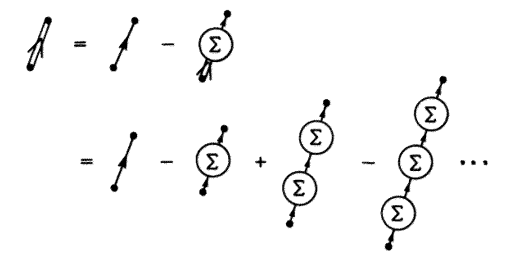
\includegraphics[width=10cm]{p17.png}
    \caption*{}
    \label{}
\end{figure}
\subsection*{Higher-order Vertex Functions}
We introduce an economical graphical representation for differentiations 
\begin{figure}[H]
    \centering
    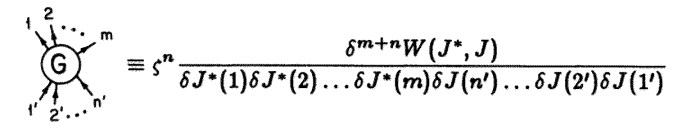
\includegraphics[width=13cm]{p18.png}
    \caption*{}
    \label{}
\end{figure}
and 
\begin{figure}[H]
    \centering
    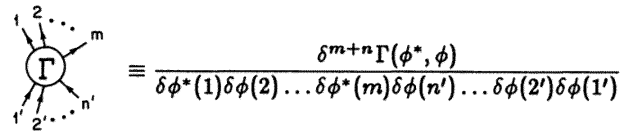
\includegraphics[width=12cm]{p19.png}
    \caption*{}
    \label{}
\end{figure}
With this notation, we can write:
\begin{figure}[H]
    \centering
    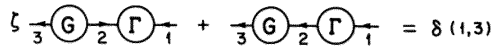
\includegraphics[width=9cm]{p20.png}
    \caption*{}
    \label{}
\end{figure}
To simplify, disregard the direction of the arrows. let $\frac{\delta}{\delta\phi}$ 
represent either $\frac{\delta}{\delta\phi(i)}$ or $\frac{\delta}{\delta\phi^*(i)}$ 
and let $\frac{\delta}{\delta J}$ represent either $\frac{\delta}{\delta J(i)}$ 
or $\frac{\delta}{\delta J^*(i)}$. Then a functional derivative $\frac{\delta}
{\delta\phi}$ applied to $\frac{\delta^n}{\delta\phi^n}\Gamma$ increases the 
number of legs by one:
\begin{figure}[H]
    \centering
    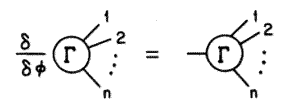
\includegraphics[width=5cm]{p21.png}
    \caption*{}
    \label{}
\end{figure}
Using the chain rule $\frac{\delta}{\delta\phi}=\frac{\delta J}{\delta\phi}
\frac{\delta}{\delta J}$, the functional derivative $\frac{\delta}{\delta\phi}$ 
applied to $\frac{\delta^n}{\delta J^n}W$ adds a leg containing $\frac{\delta
J}{\delta\phi}=\frac{\delta^2\Gamma}{\delta\phi^2}$:
\begin{figure}[H]
    \centering
    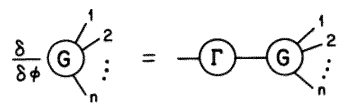
\includegraphics[width=6cm]{p22.png}
    \caption*{}
    \label{}
\end{figure}
where notice that
\begin{equation*}
    -J_\alpha(\tau)=\frac{\partial}{\partial\phi^*_\alpha(\tau)}\Gamma[\phi^*
    _\alpha(\tau),\phi_\alpha(\tau)]
\end{equation*}
With this compact notation, evaluation of $\frac{\delta^n}{\delta\phi^n}[\phi]
=\frac{\delta^n}{\delta\phi^n}[\frac{\partial W}{\partial J}]$ for successive 
values of $n$ yields the desired hierarchy of equations. For $n=1$, we get 
\begin{figure}[H]
    \centering
    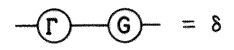
\includegraphics[width=4.5cm]{p23.jpg}
    \caption*{}
    \label{}
\end{figure}  
\subsection*{Stationary-Phase Approximation and Loop Expansion}
The stationary-phase approxiamation, also referred to as the saddle point 
approximation or method of steepest descent, is a method for developing an 
asymptotic expansion in powers of $\frac{1}{\mathcal{l}}$ for an integral of 
the form
\begin{equation*}
    I(\mathcal{l})=\int^\infty_{-\infty}dte^{-\mathcal{l}f(t)}
\end{equation*}
where $\mathcal{l}$ is a real parameter and in general f(t) ia an analytic 
function in the complex t-plane.

\end{document}